% ============================================================
% ASID 2025/2026 — Relatório Final
% Tema 2: Escalabilidade Horizontal e Custo Marginal em Microsserviços
% Grupo: PG61463, PG47542, PG58760, PG58761
% Template: ACM acmart (sigconf)
% Compilar no Overleaf ou com: pdflatex + bibtex + pdflatex x2
% ============================================================

\documentclass[manuscript,oneside]{acmart}

% --- Pacotes adicionais ---
\usepackage[portuguese]{babel}
\usepackage{booktabs}
\usepackage{multirow}
\usepackage{graphicx}
\usepackage{listings}
\usepackage{xcolor}
\usepackage{tabularx}
\usepackage{array}
\usepackage{etoolbox}
\usepackage{float}  % permite [H] para posicionamento exato de floats
% Letra menor em todas as tabelas (floats table/table*)
\AtBeginEnvironment{table}{\small}
\AtBeginEnvironment{table*}{\small}

% --- Configuração ACM ---
\acmConference[ASID 2025/2026]{Arquiteturas de Sistemas de Informação Distribuídos}{Maio 2026}{Universidade do Minho, Braga, Portugal}
\acmYear{2026}
\copyrightyear{2026}
\setcopyright{none}
\acmISBN{}
\acmDOI{}

% --- Suprimir rodapés ACM de forma limpa usando a configuração nativa ---
\settopmatter{printacmref=false, printfolios=true}
\renewcommand\footnotetextcopyrightpermission[1]{}
\pagestyle{plain}


\begin{document}

% --- Título ---
\title[Escalabilidade e Custo Marginal em Microsserviços]{Escalabilidade Horizontal e Custo Marginal em Microsserviços:\\
Um Estudo Experimental com o Google Online Boutique}

% --- Autores (Estrutura semântica oficial ACM) ---
\author{Eduardo Dias}
\email{pg61463@alunos.uminho.pt}
\affiliation{%
  \institution{Universidade do Minho}
  \department{Mestrado em Engenharia e Gestão de Sistemas de Informação}
  \city{Braga}
  \country{Portugal}
}

\author{Nuno Martinho}
\email{pg47542@alunos.uminho.pt}
\affiliation{%
  \institution{Universidade do Minho}
  \department{Mestrado em Engenharia e Gestão de Sistemas de Informação}
  \city{Braga}
  \country{Portugal}
}

\author{Clementina Kulivala}
\email{pg58760@alunos.uminho.pt}
\affiliation{%
  \institution{Universidade do Minho}
  \department{Mestrado em Engenharia e Gestão de Sistemas de Informação}
  \city{Braga}
  \country{Portugal}
}

\author{Golda Kangunga}
\email{pg58761@alunos.uminho.pt}
\affiliation{%
  \institution{Universidade do Minho}
  \department{Mestrado em Engenharia e Gestão de Sistemas de Informação}
  \city{Braga}
  \country{Portugal}
}

\renewcommand{\shortauthors}{Dias et al.}

% --- Resumo ---
\begin{abstract}
Este artigo estuda o impacto de diferentes estratégias de escalabilidade horizontal sobre o desempenho e o custo marginal de uma aplicação de microsserviços, utilizando o Google Online Boutique como sistema em estudo. Cinco cenários experimentais foram desenhados para comparar configurações de escalamento progressivamente distintas: C1 (baseline, 1 réplica), C2 (escalamento seletivo do candidato a \textit{bottleneck}), C3 (escalamento uniforme de todos os serviços \textit{stateless}), C4 (escalamento dos bottlenecks identificados empiricamente) e C5 (escalamento uniforme com proxy Envoy para balanceamento L7). Foram executados testes comparativos (15--25 utilizadores) e testes exaustivos (25--400 utilizadores) com o Locust, assumindo uma média de 3 \textit{runs} por cenário. Os resultados revelam dinâmicas contra-intuitivas: (1) O escalamento do candidato a \textit{bottleneck} (C2) antecipou a quebra para 50 utilizadores (vs.\ 75 no C1), provando que a \textit{connection affinity} do gRPC/HTTP2 torna o escalamento seletivo mal direcionado não apenas ineficaz como prejudicial; (2) Escalar os \textit{bottlenecks} reais (C4) provou ser um sucesso com custo por pedido 18\% \emph{abaixo} do baseline, sendo o único cenário mais eficiente que o C1; (3) O escalamento uniforme (C3) suportou cargas até 400 utilizadores mas com custo 17\% superior ao C1; (4) O C5, com proxy L7 Envoy, resolveu o \textit{connection affinity} (distribuição simétrica de CPU), mas o overhead do Envoy elevou o custo por pedido em 33\% face ao C1. As evidências experimentais sugerem que a identificação correta do bottleneck é o factor determinante da eficiência do escalamento horizontal em sistemas gRPC/Kubernetes, nas condições testadas.
\end{abstract}

% --- Palavras-chave ---
\keywords{microsserviços, escalabilidade horizontal, custo marginal, gRPC, \textit{connection affinity}, Kubernetes, testes de carga}

% --- Gerar cabeçalho ---
\maketitle

% ============================================================
\section{Introdução}
% ============================================================

A escalabilidade horizontal, ou seja, adicionar réplicas de serviços em vez de aumentar os recursos de uma instância, é uma das promessas centrais das arquiteturas de microsserviços. Em teoria, duplicar o número de réplicas de um serviço deveria duplicar a sua capacidade. Na prática, múltiplos fatores arquiteturais limitam este ganho: dependências de componentes \textit{stateful} partilhados, balanceamento de carga ao nível de conexão em vez de pedido, e rendimentos marginais decrescentes quando o \textit{bottleneck} se desloca para outro serviço após o escalamento.

Este trabalho analisa de que forma diferentes estratégias de escalabilidade horizontal afetam o desempenho e o custo marginal do \textit{Online Boutique}~\cite{onlineboutique}, uma aplicação de comércio eletrónico de código aberto com 11 microsserviços disponibilizada pela Google como referência de boas práticas. A escolha justifica-se por reunir características relevantes para o tema: comunicação via gRPC~\cite{grpc}, serviços \textit{stateless} e \textit{stateful}, dependências em cascata e suporte nativo a observabilidade via OpenTelemetry~\cite{otel} e Jaeger~\cite{jaeger}.

As questões de investigação que orientam o estudo são:
\begin{itemize}
  \item \textbf{RQ1:} Que serviços dominam a degradação de desempenho nos \textit{workflows} principais à medida que a carga aumenta?
  \item \textbf{RQ2:} Escalar seletivamente o serviço mais pressionado melhora de forma mensurável \textit{throughput}, latência e taxa de falhas?
  \item \textbf{RQ3:} O ganho por réplica adicional justifica o custo, ou surgem rapidamente rendimentos marginais decrescentes?
  \item \textbf{RQ4:} Até que ponto a eficácia da escalabilidade horizontal é condicionada pela natureza \textit{stateless} vs.\ dependência de componentes \textit{stateful} partilhados?
\end{itemize}

Com base nestas questões e na análise arquitetural prévia, foram formuladas seis hipóteses (H1--H6) que operacionalizam as RQs em previsões testáveis, descritas em detalhe abaixo. O estudo avalia cada hipótese através de cinco cenários experimentais controlados, comparando configurações de escalamento distintas sobre o mesmo sistema e carga.

\vspace{0.3cm}
\noindent\textbf{Repositório do Projeto:} O código fonte, \textit{scripts} de automação e registos brutos de métricas (CSV) estão integralmente disponíveis no repositório público do GitHub: \url{https://github.com/Eduardomfdias/microservices.git}
\vspace{0.3cm}

\subsection{Hipóteses de Investigação}
\label{subsec:hipoteses}

As hipóteses seguintes foram formuladas antes da execução dos testes, com base na análise arquitetural dos \textit{workflows} e nas propriedades conhecidas do sistema. Cada hipótese está associada a uma ou mais questões de investigação (RQ) e a cenários específicos que permitem testá-la. Os resultados experimentais permitem classificar cada hipótese como confirmada, inconclusiva ou fortemente suportada, conforme detalhado na Secção~\ref{sec:hipoteses-discussao}.

\textbf{H1: Escalamento seletivo com melhoria parcial.} Escalar seletivamente o \texttt{productcatalogservice} (C2) melhora parcialmente o desempenho global a carga baixa, mas não desloca o ponto de saturação se outro serviço se tornar o bottleneck dominante sob carga severa. Esta hipótese operacionaliza a RQ2: o serviço mais chamado em W1 é o candidato natural a escalamento seletivo, mas a sua aceleração pode expor outros bottlenecks. Testa-se comparando C1 e C2 nos testes comparativos (latência mediana) e exaustivos (ponto de quebra).

\textbf{H2: Redis-cart como limitação emergente.} Após aliviar a pressão sobre o \texttt{productcatalogservice}, o \texttt{redis-cart} tende a emergir como a limitação mais visível nos \textit{workflows} W2 (\textit{add-to-cart}) e W3 (\textit{checkout}), dado que é o único componente \textit{stateful} e \textit{single-threaded} do sistema. Esta hipótese operacionaliza a RQ4 e é observável via métricas de CPU/RAM do \texttt{redis-cart} nos cenários com maior carga sobre W2/W3.

\textbf{H3: Rendimentos marginais decrescentes.} O ganho de \textit{throughput} por réplica adicional tende a diminuir progressivamente à medida que o bottleneck se desloca para outras dependências não escaladas. Esta hipótese operacionaliza a RQ3 e é quantificada pelo indicador $CM_{throughput}$ comparado entre C2 ($+$2~réplicas) e C3 ($+$20~réplicas).

\textbf{H4: Custo marginal crescente.} O custo marginal por pedido com sucesso tende a aumentar quando as réplicas adicionais deixam de produzir ganhos proporcionais de \textit{throughput}. Esta hipótese distingue-se de H3 por focar no custo ($C_{proxy}$/pedido): mesmo com ganho de \textit{throughput} positivo, o custo por pedido pode crescer se as réplicas corresponderem a recursos consumidos sem proporcional aumento de capacidade útil. Operacionaliza a RQ3.

\textbf{H5: Eficácia diferenciada entre stateless e stateful.} A eficácia do escalamento horizontal é maior nos serviços \textit{stateless} do que nos cenários com dependência de um componente \textit{stateful} partilhado. Escalar o \texttt{cartservice} (stateless aplicacional) não alivia a pressão no \texttt{redis-cart} (stateful), pelo que o limite do escalamento horizontal está na capacidade do backend stateful. Operacionaliza a RQ4.

\textbf{H6: \textit{Connection affinity} como limitação estrutural.} O mecanismo de \textit{connection affinity} do gRPC/HTTP2 em Kubernetes limita estruturalmente a eficácia do escalamento horizontal sem balanceamento ao nível de pedido: as réplicas novas recebem tráfego mínimo porque as conexões HTTP/2 existentes permanecem nas réplicas originais. Esta hipótese operacionaliza as RQ1 e RQ2, sendo testada pela distribuição de CPU entre réplicas em C2 (assimetria esperada) e pela comparação C3 vs.\ C5 com Envoy L7 (resolução esperada).

\begin{table}[H]
\caption{Síntese das hipóteses, cenário principal de teste e estado após experimentação. Detalhe na Secção~\ref{sec:hipoteses-discussao}.}
\label{tab:hipoteses}
\begin{tabularx}{\columnwidth}{lXp{1.8cm}p{2.3cm}}
\toprule
\textbf{H} & \textbf{Hipótese (síntese)} & \textbf{Cenário} & \textbf{Estado} \\
\midrule
H1 & Seletivo melhora parcialmente mas pode não deslocar o ponto de quebra & C1 vs.\ C2 & \checkmark\ Confirmada \\
H2 & Redis-cart emerge como limitação após alívio do productcatalog & C2/C3 obs. & $\circ$\ Inconclusiva \\
H3 & Rendimentos marginais decrescentes por réplica adicional & C1$\to$C2$\to$C3 & \checkmark\ Confirmada \\
H4 & Custo marginal cresce quando réplicas não geram ganho proporcional & C2 vs.\ C3 & $\circ$\ Conf.\ parc. \\
H5 & Escalamento mais eficaz em stateless do que com dependência stateful & C3 vs.\ redis & $\circ$\ Inconclusiva \\
H6 & \textit{Connection affinity} gRPC/HTTP2 limita o scale-out sem L7 & C2; C3 vs.\ C5 & \checkmark\checkmark\ Fort.\ sup. \\
\bottomrule
\end{tabularx}
\end{table}

% ============================================================
\section{Enquadramento Teórico}
\label{sec:teoria}
% ============================================================

\textbf{Microsserviços e escalabilidade horizontal.} As arquiteturas de microsserviços estruturam uma aplicação como um conjunto de serviços independentemente implantáveis que comunicam por protocolos leves~\cite{fowler,newman}. A principal promessa arquitetural é a capacidade de escalar, implantar e evoluir cada serviço de forma autónoma. O \textbf{escalamento horizontal} (\textit{scale-out}), que consiste em adicionar réplicas em vez de aumentar recursos de uma instância, é a estratégia preferida porque não tem teto físico e aumenta a disponibilidade. Porém, a Lei de Amdahl~\cite{amdahl} quantifica um limite fundamental: se uma fração $s$ do trabalho é serial, o speedup máximo é $1/s$, independentemente do número de réplicas. Neste estudo, derivou-se empiricamente $s \approx 0{,}415$ para C3 sem balanceamento L7 e $s \approx 0{,}369$ com proxy Envoy (Secção~\ref{subsec:amdahl}), imposta pelo protocolo de comunicação, e não apenas pelo código.

\textbf{gRPC, HTTP/2 e \textit{connection affinity}.} O gRPC~\cite{grpc} usa HTTP/2 como transporte, com conexões persistentes e multiplexadas. Ao contrário do HTTP/1.1, onde cada pedido pode ser roteado independentemente, os pedidos gRPC partilham conexões de longa duração, uma vez que o balanceamento de carga ao nível TCP (L4) distribui conexões, não pedidos. Uma vez estabelecida uma conexão a uma réplica, todos os pedidos nessa conexão permanecem nela~\cite{grpcloadbalancing,k8sgrpc}. Este fenómeno, documentado na literatura técnica sobre gRPC em Kubernetes, é o mecanismo central que explica os resultados dos cenários C2 e C4 deste estudo.

\textbf{Kubernetes e balanceamento de carga.} O Kubernetes opera ao nível L4 através do kube-proxy (iptables/IPVS), adequado para HTTP/1.1 mas insuficiente para gRPC. A resolução requer balanceamento ao nível L7 (pedido), tipicamente fornecido por um \textit{service mesh} (Istio, Linkerd) ou por balanceamento do lado do cliente. O \textit{Horizontal Pod Autoscaler} (HPA)~\cite{k8shpa} oferece escalamento reativo, mas pressupõe que o escalamento é eficaz, um pressuposto questionado pelos resultados deste estudo.

\textbf{Componentes stateful e limite de escalabilidade.} A distinção entre serviços stateless e backends stateful é central na análise de escalabilidade. Serviços stateless podem ser replicados sem coordenação; backends stateful (bases de dados, caches) concentram estado e contenção, e a sua escalabilidade requer estratégias distintas (\textit{sharding}, replicação com consistência eventual). O \texttt{redis-cart} deste sistema é \textit{single-threaded} e não beneficia de escalamento horizontal simples, ao contrário dos 11 serviços aplicacionais.

\textbf{Observabilidade.} A identificação de bottlenecks em sistemas distribuídos requer os três pilares de observabilidade: métricas agregadas (\texttt{kubectl top}), \textit{traces} distribuídos (Jaeger/OpenTelemetry) e \textit{logs}. Neste estudo, os traces Jaeger confirmaram o fan-out ×6 de W1 e a sequencialidade total de W3; sem observabilidade, a seleção do candidato a bottleneck teria de assentar em suposições arquiteturais, como aconteceu em C2, que escalou o serviço errado com base apenas na contagem de chamadas gRPC.

\textbf{Atributos de qualidade e trade-offs arquiteturais.} A análise de decisões arquiteturais exige avaliar os impactos sobre múltiplos atributos de qualidade em simultâneo. Neste estudo, seguem-se quatro atributos centrais: \textbf{Performance} (throughput, latência, ponto de saturação), \textbf{Availability} (redundância, eliminação de pontos únicos de falha), \textbf{Deployability} (complexidade operacional, esforço de configuração e manutenção) e \textbf{Cost} (consumo de recursos, custo por pedido). Qualquer decisão de escalamento horizontal afeta estes quatro atributos de forma interdependente: adicionar réplicas pode melhorar Performance e Availability mas aumentar Cost e complexidade de Deployability~\cite{newman}.

\textbf{Custo operacional e custo proxy em sistemas cloud-native.} Em ambientes cloud-native, o custo operacional de uma configuração é tipicamente proporcional ao consumo de CPU e memória ao longo do tempo. Na ausência de dados de faturação real (ambiente local), este estudo usa um \textit{proxy} analítico: $C_{proxy} = \alpha \cdot CPU_{time} + \beta \cdot RAM_{time}$, onde $CPU_{time}$ e $RAM_{time}$ são o consumo médio acumulado ao longo do teste. O custo marginal por pedido ($C_{proxy}/pedidos_{sucesso}$) permite comparar a eficiência de diferentes configurações de escalamento. Este índice é relativo e não representa grandeza monetária ou física absoluta, sendo o seu valor relevante apenas para comparação entre cenários.

\textbf{Comparação com sistemas de produção.} A \textbf{Netflix} resolveu o mesmo problema de \textit{connection affinity} com balanceamento do lado do cliente (Ribbon/Envoy). A \textbf{Twitter/X} enfrentou os mesmos limites de componentes stateful (Redis) ao migrar para microsserviços, recorrendo a \textit{sharding} e separação de leituras/escritas. A \textbf{Amazon} opera com escalamento por serviço independente, mas enfatiza que o escalamento de um serviço aumenta a carga nos seus dependentes, reproduzindo exatamente o efeito cascata observado no C4 deste estudo.

% ============================================================
\section{Contexto e Arquitetura Relevante}
% ============================================================

O \textit{Online Boutique} é composto por 11 microsserviços e um componente \textit{stateful} (Redis). A arquitetura segue o padrão \textit{Database-per-Service}, onde apenas o \texttt{redis-cart} mantém estado persistente. Todos os serviços aplicacionais são \textit{stateless}. A comunicação interna é exclusivamente via gRPC sobre HTTP/2; o único ponto de entrada externo é o \texttt{frontend}, que expõe HTTP/1.1.

\textbf{Nota conceptual importante:} o \texttt{cartservice} é um serviço aplicacional \textit{stateless} que depende de um \textit{backend stateful} partilhado (\texttt{redis-cart}). Escalar réplicas do \texttt{cartservice} não escala o recurso que concentra o estado e a contenção. Esta distinção é central para a interpretação dos resultados.

O inventário completo dos 11 microsserviços, detalhando linguagem, porta, tipo e responsabilidade, encontra-se no Anexo~\ref{apx:inventario} (Tabela~\ref{tab:inventario}). O diagrama de dependências entre serviços encontra-se no Anexo~\ref{apx:dependencias} (Figura~\ref{fig:dependencias}).

\subsection{Workflows Analisados}

Foram selecionados três \textit{workflows} que cobrem padrões distintos de escalabilidade.

\textbf{W1: Browse Product} (\texttt{GET /product/\{id\}}): desencadeia 6 chamadas gRPC paralelas ao \texttt{productcatalogservice} por pedido, conforme confirmado com traces Jaeger. É a operação mais frequente (peso~10 no Locust) e o principal \textit{driver} de carga do \texttt{productcatalogservice}.

\textbf{W2: Add to Cart} (\texttt{POST /cart}): envolve validação do produto e persistência no \texttt{redis-cart} via HSET bloqueante. É pré-requisito funcional do \textit{checkout}: falha aqui bloqueia W3 em 100\% dos casos.

\textbf{W3: Checkout} (\texttt{POST /cart/checkout}): o \texttt{checkoutservice} orquestra 6 serviços em sequência, pelo que a latência total é a soma das latências individuais, sem paralelismo. A operação EmptyCart ocorre no final, após \textit{checkout} bem-sucedido (confirmado no Jaeger).

Os diagramas de sequência detalhados de W1, W2 e W3 encontram-se no Anexo~\ref{apx:sequencias} (Figuras~\ref{fig:seq-w1}, \ref{fig:seq-w2} e~\ref{fig:seq-w3}).

\subsection{Tabela Chamada $\rightarrow$ Dependências $\rightarrow$ Risco}

\begin{table}[H]
\caption{Análise de risco por chamada nos três workflows. Risco: ALTO = caminho crítico com fan-out, dependência \textit{stateful} ou bloqueio em cascata.}
\label{tab:risco}
\begin{tabular}{llllll}
\toprule
\textbf{WF} & \textbf{Chamada} & \textbf{Origem} & \textbf{Destino} & \textbf{Fan-out} & \textbf{Risco} \\
\midrule
W1 & GET /product     & Locust          & frontend          & —                & ALTO \\
W1 & GetProduct (×6)  & frontend        & productcatalog    & 6 paralelas      & ALTO \\
W1 & GetCurrencies    & frontend        & currencyservice   & 1                & MÉDIO \\
W1 & ListRec.         & frontend        & recommendation    & 1 (chama cat.)   & BAIXO \\
W2 & POST /cart       & Locust          & frontend          & 2 sequenciais    & ALTO \\
W2 & GetProduct       & frontend        & productcatalog    & 1                & MÉDIO \\
W2 & AddItem (HSET)   & frontend        & cart→redis        & 1 bloqueante     & ALTO \\
W3 & POST /checkout   & Locust          & frontend→checkout & 6 sequenciais    & ALTO \\
W3 & GetCart          & checkoutservice & cart→redis        & 1                & ALTO \\
W3 & Charge           & checkoutservice & paymentservice    & 1                & ALTO \\
W3 & SendEmail        & checkoutservice & emailservice      & 1                & BAIXO \\
W3 & EmptyCart        & checkoutservice & redis-cart        & 1                & MÉDIO \\
\bottomrule
\end{tabular}
\end{table}

\subsection{Serviços-Alvo}

Com base na análise de fan-out, tipo de estado e presença nos três \textit{workflows}, foram selecionados três serviços-alvo para orientar os cenários experimentais.

\begin{table}[H]
\caption{Serviços-alvo selecionados (ST1--ST3), tipo, cenário de escala e justificação.}
\label{tab:alvos}
\begin{tabularx}{\columnwidth}{p{2cm}p{1.4cm}p{1.7cm}X}
\toprule
\textbf{Serviço-alvo} & \textbf{Tipo} & \textbf{Cenário} & \textbf{Justificação} \\
\midrule
ST1: \texttt{productcatalog} & Stateless & C2 (×3 répl.) & Fan-out ×6 em W1, sem cache, chamado em W1/W2/W3. Stateless; escalamento seguro. Testa RQ1 e RQ2. \\
\addlinespace
ST2: \texttt{redis-cart} & Stateful & C1/C2 (obs.) & Único componente stateful; single-threaded. Escalar o \texttt{cartservice} não resolve a pressão no \texttt{redis-cart}. Testa RQ4. \\
\addlinespace
ST3: \texttt{frontend} & Stateless & C3 (uniforme) & Ponto de entrada único. O C3 isola se o gargalo está na receção HTTP ou nas dependências internas. \\
\bottomrule
\end{tabularx}
\end{table}

% ============================================================
\section{Decisão Arquitetural em Estudo}
% ============================================================

A decisão arquitetural central deste estudo é a \textbf{estratégia de escalamento horizontal}: escalar \emph{seletivamente} apenas o(s) serviço(s) candidatos a \textit{bottleneck} (C2), por oposição a escalar \emph{uniformemente} todos os serviços \textit{stateless} (C3). Esta decisão é avaliada experimentalmente nos cenários descritos na Secção~\ref{sec:metodologia}.

A motivação para estudar esta decisão decorre de uma tensão arquitetural real: o escalamento seletivo é aparentemente mais eficiente (menos réplicas, menor custo), mas exige identificação prévia do bottleneck; o escalamento uniforme é operacionalmente mais simples mas ignora diferenças de carga entre serviços. A escolha entre estas estratégias tem impacto direto nos quatro atributos de qualidade em avaliação: \textbf{Performance}, \textbf{Availability}, \textbf{Deployability} e \textbf{Cost}.

Um fator arquitetural crítico condiciona ambas as estratégias: a \textit{connection affinity} do gRPC/HTTP2~\cite{grpcloadbalancing,k8sgrpc}. O gRPC usa conexões persistentes e multiplexadas. Uma vez estabelecida uma conexão a uma réplica, todos os pedidos nessa conexão continuam a ir para a mesma réplica. Novas réplicas só recebem tráfego quando novas conexões são abertas. Este comportamento, documentado na literatura técnica sobre balanceamento gRPC em Kubernetes~\cite{k8sgrpc}, limita estruturalmente a eficácia do escalamento horizontal simples (\texttt{kubectl scale}) em sistemas gRPC, independentemente da estratégia adotada.

\subsection{Alternativas Consideradas à Decisão de Escalamento Estático}

As alternativas seguintes foram analisadas e descartadas ou não implementadas no âmbito deste estudo. A sua discussão é relevante para contextualizar a decisão arquitetural tomada (escalamento estático por \texttt{kubectl scale}) e para identificar caminhos de evolução. Nenhuma destas alternativas foi objeto de teste experimental; a sua avaliação é baseada em análise arquitetural e literatura.

\textbf{Auto-scaling horizontal (HPA por CPU/memória).} O Kubernetes \textit{Horizontal Pod Autoscaler}~\cite{k8shpa} ajusta o número de réplicas automaticamente com base em métricas. Melhora a \textbf{Performance} ao reagir à carga real; melhora a \textbf{Availability} sob carga variável; aumenta a complexidade de \textbf{Deployability} (requer configuração de métricas, limiares e políticas de \textit{cooldown}); o \textbf{Cost} é variável: potencialmente menor em períodos calmos, com risco de \textit{over-provisioning} em rajadas.

\textbf{Caching no productcatalogservice.} Introduzir uma cache em memória ou via Redis eliminaria o fan-out de 6 chamadas por browse, reduzindo drasticamente a pressão no serviço. Melhoria substancial de \textbf{Performance} sem adição de réplicas; \textbf{Availability} pode ser afetada por inconsistências de TTL; exige alteração de código (\textbf{Deployability} média); \textbf{Cost} potencialmente muito inferior ao escalamento (sem réplicas extras).

\textbf{Service mesh com balanceamento por pedido (Istio/Linkerd).} Um \textit{service mesh}~\cite{servicemesh} introduz um proxy \textit{sidecar} (ex: Envoy) em cada pod, funcionando como middleware acima do Kubernetes ao nível L7. Este middleware intercepta todo o tráfego gRPC e substitui o balanceamento por conexão por balanceamento por pedido (\textit{round-robin} ou \textit{least-connections}), resolvendo estruturalmente a \textit{connection affinity} identificada em H6~\cite{k8sgrpc}. Impacto nos atributos de qualidade: melhoria substancial de \textbf{Performance} ao distribuir carga uniformemente, fazendo com que as réplicas novas passem a receber tráfego imediatamente, sem aguardar novas conexões; melhoria de \textbf{Availability} com \textit{circuit breaking}, \textit{retry} automático e deteção de réplicas degradadas; aumento significativo de complexidade operacional (\textbf{Deployability}), dado que o service mesh adiciona um componente de infraestrutura com a sua própria curva de aprendizagem, configuração e potencial de falha; overhead de CPU/memória do sidecar ($\sim$20--50~m por pod) impacta o \textbf{Cost}. Esta é a alternativa não implementada com maior potencial para resolver o problema central identificado neste estudo.

\textbf{Escalamento vertical (ajuste de limites de recursos).} Aumentar CPU/RAM dos pods existentes em vez de adicionar réplicas. Simplicidade máxima de \textbf{Deployability}; \textbf{Performance} limitada pelo teto do nó; \textbf{Availability} sem melhoria (sem redundância); \textbf{Cost} proporcional aos recursos alocados.

\subsection{Trade-offs: Escalamento Seletivo vs. Uniforme}

\begin{table}[H]
\caption{Trade-offs da decisão central (C2 vs.\ C3) por atributo de qualidade.}
\label{tab:tradeoffs}
\begin{tabular}{p{1.8cm}p{2.8cm}p{2.8cm}}
\toprule
\textbf{Atributo} & \textbf{Seletivo (C2)} & \textbf{Uniforme (C3)} \\
\midrule
Performance & Ganho na latência mediana ($-22\%$ p50). Risco: se o bottleneck não for o serviço escalado, pode degradar (C2 $<$ C1 nos exaustivos, quebra a 50u) & Maior ponto de saturação ($>$400u vs 75u). Sem melhoria na mediana. \\
\addlinespace
Availability & Serviços não escalados permanecem pontos únicos de falha & Redundância em todos os stateless; redis-cart é o único ponto único \\
\addlinespace
Deployability & Requer identificação prévia do bottleneck (tracing, análise de CPU) & Mecânico, sem análise prévia; mais réplicas = mais complexidade de gestão \\
\addlinespace
Cost & Menor custo absoluto (+2 réplicas); custo marginal negativo se mal direcionado & Custo 3× superior (+20 réplicas); ganho no ponto de saturação justifica parcialmente \\
\bottomrule
\end{tabular}
\end{table}

A evidência experimental mostra que o escalamento seletivo (C2) é a decisão de maior risco: quando o serviço identificado como candidato a \textit{bottleneck} não é o \textit{bottleneck} real sob carga severa, as réplicas adicionais consomem recursos sem receber tráfego (efeito da \textit{connection affinity} gRPC), degradando o sistema. O escalamento uniforme (C3) é mais robusto mas com custo marginal crescente.

% Hipóteses movidas para a secção de Introdução como subsecção, conforme estrutura sugerida pela professora.

% ============================================================
\section{Desenho Experimental}
\label{sec:metodologia}
% ============================================================

\subsection{Ambiente}

Os testes foram executados num MacBook Air M4 (2026): Apple M4 10 cores (4P+6E), 16~GB RAM. O Kubernetes foi gerido pelo Docker Desktop, com o nó único a receber todos os 10 cores e $\sim$7,6~GB de RAM. O ambiente local impõe limitações face a um cluster de produção (sem isolamento NUMA, variabilidade de processos do SO), devidamente consideradas na análise.

Foram necessários dois ajustes para Apple Silicon ARM64: aumento do \textit{memory limit} do \texttt{cartservice} de 128~MiB para 512~MiB (evitar OOMKill sob carga) e a variável de ambiente \texttt{DOTNET\_EnableWriteXorExecute=0} (corrigir \textit{crash} do JIT .NET em ARM64). Todos os \textit{deployments} usam \texttt{imagePullPolicy: Never}, sendo as imagens construídas e \textit{tagged} localmente.

\subsection{Ferramenta de Carga: Locust}

A carga foi gerada com Locust~\cite{locust} (Python), ferramenta incluída no projeto original. Foram implementados dois \textit{locustfiles} com perfis de utilizador distintos.

\textbf{Locustfile comparativo} (think times realistas): CasualUser~30\%/5--15s, NormalUser~50\%/2--6s, PowerUser~20\%/0,5--2s. A 25 utilizadores gera $\approx$8~RPS, o que se revela insuficiente para saturar o sistema.

\textbf{Locustfile exaustivo} (think times agressivos): CasualUser~20\%/0,5--1s, NormalUser~50\%/0,2--0,5s, PowerUser~30\%/0,1--0,2s. A 25 utilizadores gera $\approx$72~RPS. Permite encontrar o ponto de saturação real.

A existência de dois perfis distintos reflete papéis complementares: o comparativo permite comparar C1, C2 e C3 em condições controladas e equivalentes, a carga sub-saturação; o exaustivo procura forçar a saturação para identificar o ponto de rutura real de cada cenário. As inferências sobre throughput máximo sustentável e custo por pedido provêm exclusivamente do segundo perfil. \textbf{Os resultados dos dois conjuntos de testes não são diretamente comparáveis entre si}, devido à utilização de locustfiles diferentes e objetivos distintos.

Pesos das tarefas (ambos): \texttt{browse×10 · view-cart×3 · add-to-cart×2 · moeda×2 · homepage×1 · checkout×1}. O workload não representa um único workflow isolado, mas uma composição de operações sobre a aplicação cuja interpretação deve ser feita à luz de W1 (principal driver de fan-out sobre o \texttt{productcatalogservice}), W2 (workflow associado ao carrinho e ao backend stateful) e W3 (workflow transacional de maior complexidade e latência acumulada). O \textit{checkout} usa \texttt{catch\_response=True} para não contaminar as métricas com falhas provenientes do \textit{add-to-cart}. O \texttt{loadgenerator} nativo foi pausado (\texttt{kubectl scale --replicas=0}) em todas as execuções.

\subsection{Cenários Experimentais}

\begin{table}[H]
\caption{Descrição dos cenários experimentais.}
\label{tab:cenarios}
\begin{tabularx}{\columnwidth}{lXlX}
\toprule
\textbf{Cenário} & \textbf{Configuração} & \textbf{+Comp.} & \textbf{Objetivo} \\
\midrule
C1 & 1 réplica por serviço & 0 & Referência; ponto de saturação natural \\
C2 & productcatalog: 3; restantes: 1 & +2 & Escalar candidato a bottleneck primário \\
C3 & Todos stateless: 3; redis-cart: 1 & +20 & Escalar tudo; rendimentos marginais? \\
C4 & frontend: 3; currency: 3; restantes: 1 & +4 & Escalar os bottlenecks reais identificados \\
C5 & Todos stateless: 3 + Envoy proxy L7 & +20+Envoy & Mitigar connection affinity; validar H6 \\
\bottomrule
\end{tabularx}
\end{table}

\textbf{Parâmetros de execução:} warm-up de 30~s (permite estabilização inicial do sistema antes da recolha); janela de medição de 120~s por nível (observar o sistema num período relativamente estável); spawn rate 2~utilizadores/s (evitar subida demasiado brusca da carga); cooldown 60~s entre níveis. O critério de quebra (p99~>~2000~ms OU falhas~>~5\%) é um limiar operacional consistente para identificar degradação severa e tornar comparável o ponto de rutura entre cenários, não representando um Service Level Agreement real da aplicação.

\textbf{Testes comparativos:} cargas fixas 15, 20, 25 utilizadores; locustfile realista; cada execução independente com cluster em estado limpo. Este isolamento entre execuções permite comparação rigorosa entre cenários à mesma carga.

\textbf{Testes exaustivos:} carga crescente 25→50→75→100→125→150 utilizadores dentro da \emph{mesma execução}; locustfile agressivo; execução até ao critério de quebra ser atingido. O \textit{cooldown} de 60~s reduz a transição abrupta mas não elimina efeitos herdados do nível anterior (conexões gRPC aquecidas, JIT compilado). O ponto de saturação assim obtido deve ser interpretado como indicativo de tendência de degradação, não como equivalente a execuções independentes por nível de carga.

\subsection{Contexto Histórico: C1 Exploratório}

Antes dos testes comparativos foi executado um teste exploratório de C1 com um \textit{locustfile} simplificado (1 perfil, \texttt{wait\_time} entre(0{,}5,1)) com carga crescente progressiva, para identificar o ponto de saturação do sistema e calibrar os níveis de carga. \textbf{Estes resultados não são comparáveis com os testes comparativos}, dada a utilização de um locustfile diferente e de uma metodologia distinta.

\begin{table}[H]
\caption{C1 Exploratório (locustfile simplificado, carga crescente). Saturação a 30 utilizadores com 47{,}6\% de falhas, o que motivou a escolha de 15/20/25 utilizadores para os testes comparativos.}
\label{tab:c1exp}
\begin{tabular}{lrrrrrrl}
\toprule
\textbf{Users} & \textbf{p50} & \textbf{p90} & \textbf{p99} & \textbf{Falhas\%} & \textbf{RPS} & \textbf{Estado} \\
\midrule
5  & 25ms & 36ms  & 130ms & 0{,}0\% & 1{,}71 & OK \\
10 & 21ms & 36ms  & 77ms  & 0{,}0\% & 3{,}41 & OK \\
15 & 22ms & 35ms  & 120ms & 0{,}0\% & 4{,}98 & OK \\
20 & 26ms & 120ms & 410ms & 0{,}0\% & 6{,}60 & Aviso (p90 sobe 3×) \\
25 & 21ms & 65ms  & 420ms & 0{,}0\% & 8{,}35 & Aviso \\
\textbf{30} & \textbf{13ms} & \textbf{210ms} & \textbf{910ms} & \textbf{47{,}6\%} & \textbf{8{,}79} & \textbf{SATURAÇÃO} \\
\bottomrule
\end{tabular}
\end{table}

A degradação do p90 entre 15 e 20 utilizadores (36\,ms~$\rightarrow$~120\,ms, aumento de 3$\times$) e a posterior saturação a 30 utilizadores (47{,}6\% de falhas HTTP~422, maioritariamente no \textit{checkout} em cascata a partir de falhas no \textit{add-to-cart}) motivaram a escolha dos níveis 15, 20 e 25 utilizadores para os testes comparativos, abrangendo o intervalo de degradação progressiva até ao limite antes da quebra, sem atingir saturação completa.

\subsection{Métricas Recolhidas}

Throughput (RPS), latências p50/p90/p99 e taxa de falhas foram exportados pelo Locust em CSV. CPU e RAM por pod a cada 10s durante os testes via \texttt{kubectl top}, guardados em \texttt{monitoring/pods\_metrics.csv}. Traces distribuídos via Jaeger para análise de dependências e ordem das chamadas.

\subsection{Definição Operacional de Custo Marginal}

\[
CM_{throughput} = \frac{\Delta RPS}{\Delta R\acute{e}plicas}
\qquad
C_{proxy} = \frac{1}{2} \cdot CPU_{time} + \frac{1}{2} \cdot RAM_{time}
\]

onde $CPU_{time} = \overline{cpu_{m}} / 1000 \times t_{s}$ (CPU-segundos por réplica) e $RAM_{time} = \overline{ram_{MiB}} \times t_{s}$ (MiB-segundos por réplica), somados sobre todas as réplicas do cenário. O custo por pedido com sucesso é $C_{proxy} / pedidos_{sucesso}$, permitindo comparar cenários com throughputs diferentes.

\textbf{Nota sobre as métricas:} $CM_{throughput}$ mede o ganho de \textit{throughput} por réplica adicional, sendo um indicador de eficiência de escalamento, não de custo diretamente. O custo marginal é capturado pelo $C_{proxy}$ e pelo custo por pedido. Os pesos $\alpha = \beta = 0{,}5$ são uma escolha metodológica simplificadora para construir um indicador comparável entre cenários; as duas grandezas (CPU-s e MiB-s) têm unidades distintas e a sua soma não tem significado físico direto fora deste contexto comparativo. O $C_{proxy}$ é um índice relativo, não uma grandeza monetária ou física absoluta.

Os valores de CPU e RAM foram obtidos a partir dos ficheiros \texttt{pods\_after.txt} (medição pontual \texttt{kubectl top} no final de cada nível de carga), usando a média das três medições (15/20/25 utilizadores) × 120\,s de janela de medição por nível. A Tabela~\ref{tab:custo} apresenta os resultados calculados.

\begin{table}[H]
\caption{Custo proxy calculado para C1, C2 e C3 (testes comparativos, 15/20/25 utilizadores, $t_{total}=360$\,s). CPU\_time em CPU-s; RAM\_time em MiB-s; $C_{proxy} = 0{,}5\times\text{CPU}_{time} + 0{,}5\times\text{RAM}_{time}$; custo/req em unidades proxy por pedido com sucesso.}
\label{tab:custo}
{\footnotesize
\begin{tabular}{lrrrrrrrr}
\toprule
\textbf{Cenário} & \textbf{+Rép.} & \textbf{CPU\_t} & \textbf{RAM\_t} & \textbf{$C_{proxy}$} & \textbf{Req OK} & \textbf{C/req} & \textbf{$\Delta$C/req} & \textbf{$CM_{tp}$} \\
\midrule
C1: Baseline & 0   & 59{,}8 & 353\,640 & 176\,850 & 2285 & 77{,}4 & — & — \\
C2: Seletivo & +2  & 86{,}3 & 370\,560 & 185\,323 & 2301 & 80{,}5 & $+$4\%   & $-$0{,}02 \\
C3: Uniforme & +20 & 84{,}2 & 817\,320 & 408\,702 & 2300 & 177{,}7 & $+$130\% & $-$0{,}003 \\
\bottomrule
\end{tabular}%
}
\end{table}

\textbf{Leitura:} o C2 adicionou 2 réplicas e aumentou o custo por pedido apenas 4\%, mas sem qualquer ganho de throughput ($CM_{tp}=-0{,}02$~RPS/réplica). O C3 adicionou 20 réplicas (+182\% de pods) e o custo por pedido subiu 130\%, com throughput marginalmente inferior ao C1 ($CM_{tp}=-0{,}003$~RPS/réplica). O RAM\_time domina o custo proxy porque a RAM alocada é proporcional ao número de réplicas, enquanto a CPU real consumida é condicionada pela \textit{connection affinity} (réplicas ociosas consomem pouca CPU mas continuam a ocupar RAM).

% ============================================================
\section{Resultados}
\label{sec:resultados}

\subsection{Testes Comparativos}
\label{sec:comparativos}
% ============================================================

Os testes comparativos usaram o locustfile realista a 15, 20 e 25 utilizadores. A carga de 25 utilizadores não saturou nenhum dos três cenários. A Tabela~\ref{tab:comparativos} apresenta os resultados agregados; a Tabela~\ref{tab:cpu} detalha a distribuição de CPU por réplica.

\begin{table}[H]
\caption{Resultados comparativos C1, C2 e C3 (testes com locustfile realista). A carga de 25 utilizadores não satura nenhum cenário, sendo o throughput praticamente idêntico ($\approx$8~RPS).}
\label{tab:comparativos}
\begin{tabular}{lrrrrrr}
\toprule
\textbf{Users} & \textbf{p50} & \textbf{p90} & \textbf{p99} & \textbf{Falhas\%} & \textbf{RPS} \\
\midrule
\multicolumn{6}{l}{\textit{C1: Baseline (1 réplica por serviço)}} \\
15 & 20ms & 30ms & 62ms & 0,0\% & 4,80 \\
20 & 18ms & 31ms & 52ms & 0,0\% & 6,36 \\
25 & 18ms & 31ms & 69ms & 0,0\% & 7,98 \\
\midrule
\multicolumn{6}{l}{\textit{C2: Seletivo (productcatalogservice ×3)}} \\
15 & 16ms & 27ms & 170ms & 0,0\% & 4,92 \\
20 & 16ms & 25ms & 86ms & 0,0\% & 6,42 \\
25 & 14ms & 25ms & 290ms & 0,0\% & 7,94 \\
\midrule
\multicolumn{6}{l}{\textit{C3: Uniforme (todos stateless ×3; redis-cart ×1)}} \\
15 & 21ms & 38ms & 200ms & 0,0\% & 4,78 \\
20 & 19ms & 32ms & 96ms & 0,0\% & 6,57 \\
25 & 19ms & 31ms & 110ms & 0,0\% & 7,92 \\
\bottomrule
\end{tabular}
\end{table}

Como se observa na Tabela~\ref{tab:comparativos}, os resultados revelam três padrões consistentes.

\textbf{Throughput:} praticamente idêntico nos 3 cenários ($\approx$7,9--8,0~RPS a 25 utilizadores). O escalamento não produz ganho de throughput porque o sistema não está saturado, o que se revela um resultado consistente com H3 e H4 nesta gama de carga.

\textbf{Latência mediana (p50):} o C2 apresenta a melhor mediana (14~ms a 25u, $-22\%$ face ao C1). Este ganho é compatível com uma distribuição parcial de carga no \texttt{productcatalogservice} quando novas conexões são abertas.

\textbf{Latência cauda (p99):} o C1 tem os melhores p99. O C2 e C3 mostram picos mais altos (290~ms e 110~ms vs.\ 69~ms no C1 a 25u), padrão que se revela consistente com réplicas novas menos ``aquecidas'' (JIT não otimizado, caches frias) e com a hipótese de H6.

Como se observa na Tabela~\ref{tab:cpu}, a distribuição de CPU no C2 revela: \texttt{productcatalogservice} \#1: 31m | \#2: 2m | \#3: 1m, com uma distribuição de 91\%/6\%/3\%. As duas réplicas novas ficaram praticamente inativas porque as conexões HTTP/2 existentes permaneceram na réplica original, numa observação fortemente sugerida pela hipótese H6 (\textit{connection affinity} gRPC/HTTP2).

\begin{table}[htbp]
\caption{Distribuição de CPU por serviço e por réplica nos três cenários a 25 utilizadores (valores \texttt{kubectl top}, em millicores). Evidencia a \textit{connection affinity} gRPC (H6): réplicas novas ficam subutilizadas enquanto a original acumula carga.}
\label{tab:cpu}
\begin{tabularx}{\columnwidth}{lrrX}
\toprule
\textbf{Serviço} & \textbf{C1} & \textbf{C2} & \textbf{C3: todos stateless ×3} \\
\midrule
frontend              & 50m & 70m (1 répl.)               & $\sim$16m+17m+16m (uniforme) \\
currencyservice       & 47m & 55m (1 répl.)               & $\sim$26m+17m+2m (desigual) \\
recommendationservice & 31m & 47m (1 répl.)               & $\sim$39m distribuídos \\
productcatalogservice & 21m & \#1:31m | \#2:2m | \#3:1m  & $\sim$14m+7m+3m (desigual) \\
cartservice           & 23m & 23m (1 répl.)               & $\sim$29m distribuídos \\
redis-cart (stateful) & 4m  & 5m (inalterado)             & 4m (inalterado) \\
\bottomrule
\end{tabularx}
\end{table}

\begin{figure}[H]
  \centering
  
\includegraphics[width=0.6\linewidth]{figuras/fig_distribuicao_cpu_c2.pdf}
  \caption{Distribuição de CPU entre as 3 réplicas do \texttt{productcatalogservice} em C2 a 25u (testes comparativos). A réplica original absorve 91,2\% do tráfego (31m vs.\ 2m e 1m), servindo de evidência empírica da \textit{connection affinity} gRPC/HTTP2 (H6).}
  \label{fig:distrib-cpu}
\end{figure}

\begin{figure}[H]
  \centering
  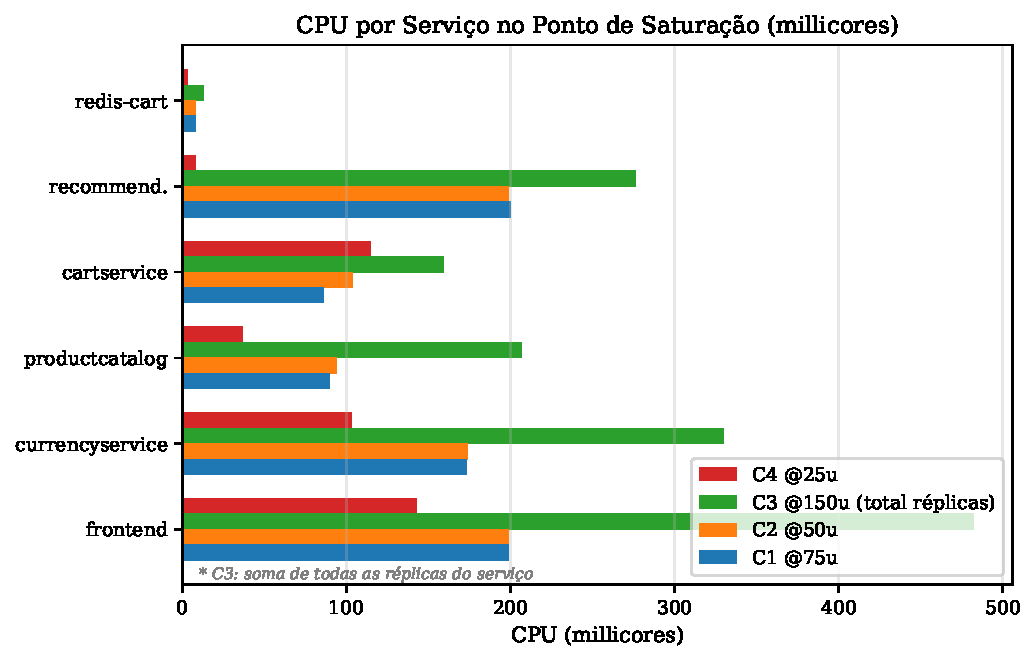
\includegraphics[width=0.85\linewidth]{figuras/fig_cpu_servicos.pdf}
  \caption{CPU total por serviço (millicores) no ponto de operação de cada cenário (médias de 3 execuções). C4 @400u mostra \texttt{frontend} e \texttt{currencyservice} escalados (×3); restantes com 1 réplica.}
  \label{fig:cpu-servicos}
\end{figure}

O \texttt{frontend} é o único serviço que distribui bem a carga em C3 ($\sim$16m+17m+16m), porque recebe conexões HTTP/1.1 externas, pelo que, sem persistência HTTP/2, cada pedido pode ser roteado independentemente. Todos os outros serviços exibem distribuição desigual entre réplicas, resultado consistente com a \textit{connection affinity} como fenómeno estrutural do gRPC/HTTP2 e não específico de um serviço em particular.

% ============================================================
\subsection{Resultados por Workflow (25 utilizadores, testes comparativos)}
\label{sec:por-workflow}
% ============================================================

A Tabela~\ref{tab:por-workflow} apresenta a latência por workflow e cenário a 25 utilizadores (médias de 3 execuções, sistema não saturado, falhas = 0\% em todos os casos). O mapeamento endpoint\,→\,workflow é: \texttt{GET /product/[id]}\,$\to$\,W1; \texttt{POST /cart [add]}\,$\to$\,W2; \texttt{POST /cart/checkout}\,$\to$\,W3.

\begin{table}[H]
\caption{Latência p50 e p99 por workflow e cenário a 25 utilizadores (médias de 3 execuções). C2 melhora W1 na mediana mas não W2, confirmando que escalar o \texttt{productcatalogservice} não beneficia o percurso crítico de W2 (\texttt{redis-cart}).}
\label{tab:por-workflow}
\begin{tabularx}{\columnwidth}{llrrrrr}
\toprule
\textbf{WF} & \textbf{Endpoint} & \multicolumn{2}{c}{\textbf{C1}} & \multicolumn{2}{c}{\textbf{C2}} & \textbf{C3} \\
\cmidrule(lr){3-4}\cmidrule(lr){5-6}
 & & \textbf{p50} & \textbf{p99} & \textbf{p50} & \textbf{p99} & \textbf{p50 / p99} \\
\midrule
W1 & GET /product/[id]   & 19ms & 660ms & 18ms & 413ms & 11ms / 539ms \\
W2 & POST /cart [add]    & 27ms & 753ms & 28ms & 480ms & 16ms / 590ms \\
W3 & POST /cart/checkout & 33ms & 166ms & 33ms & 153ms & 18ms / 147ms \\
\bottomrule
\end{tabularx}
\end{table}

Como se observa na Tabela~\ref{tab:por-workflow}, cada workflow revela um padrão diferente face ao escalamento.

\textbf{W1 (Browse Product):} o C2 melhora marginalmente o p50 ($-5\%$, de 19 para 18~ms) e reduz o p99 de 660 para 413~ms, resultado compatível com a transferência parcial de carga quando novas conexões são abertas para réplicas do \texttt{productcatalogservice}. O C3 atinge o melhor p50 (11~ms, $-42\%$ face ao C1).

\textbf{W2 (Add to Cart):} o C2 não melhora o p50 de W2 (27~ms vs.\ 28~ms), o que é consistente com a expectativa arquitetural: escalar o \texttt{productcatalogservice} não afeta o percurso crítico de W2, que passa por \texttt{cartservice}\,$\to$\,\texttt{redis-cart}. O C3 melhora o p50 em $-41\%$ (16~ms).

\textbf{W3 (Checkout):} W3 apresenta os melhores p99 absolutos nos três cenários porque é o workflow menos frequente (peso~1 no Locust) e a sua latência é dominada pela soma sequencial das 6 chamadas gRPC, não pela concorrência. C2 e C3 melhoram marginalmente o p99 (166~ms\,$\to$\,153~ms e 147~ms).

\textbf{Observação transversal:} a melhoria do C2 na p50 de W1 ($-5\%$) confirma que o escalamento do \texttt{productcatalogservice} tem impacto localizado no workflow mais dependente desse serviço, sem efeito relevante em W2, cujo bottleneck é estruturalmente distinto (\texttt{redis-cart}). Este resultado é consistente com H2 e com a análise de risco da Tabela~\ref{tab:risco}.

A Tabela~\ref{tab:por-workflow-quebra} detalha o comportamento por workflow no ponto de quebra de C1 e C2.

\begin{table}[H]
\caption{Resultados por workflow no ponto de quebra: C1 a 75u e C2 a 50u (médias de 3 execuções). W1 e W2 concentram as falhas; W3 mantém-se estável porque só falha quando o carrinho já está corrompido.}
\label{tab:por-workflow-quebra}
\begin{tabularx}{\columnwidth}{llrrrr}
\toprule
\textbf{WF} & \textbf{Endpoint} & \multicolumn{2}{c}{\textbf{C1 @75u}} & \multicolumn{2}{c}{\textbf{C2 @50u}} \\
\cmidrule(lr){3-4}\cmidrule(lr){5-6}
 & & \textbf{p50} & \textbf{Falhas\%} & \textbf{p50} & \textbf{Falhas\%} \\
\midrule
W1 & GET /product/[id]   & 203ms & 23,7\% & 106ms & 9,6\% \\
W2 & POST /cart [add]    & 237ms & 25,6\% & 133ms & 10,1\% \\
W3 & POST /cart/checkout & 240ms & 0,2\%  & 131ms & 0,0\% \\
\bottomrule
\end{tabularx}
\end{table}

Como se observa na Tabela~\ref{tab:por-workflow-quebra}, no ponto de quebra de C1 (75u), as falhas concentram-se em W1 ($23{,}7\%$) e W2 ($25{,}6\%$), enquanto W3 mantém $0{,}2\%$ de falhas. Esta assimetria reflete o mecanismo de propagação: os erros HTTP~422 em W2 (\textit{add-to-cart}) impossibilitam a execução de W3 (\textit{checkout}), mas W3 apenas falha quando o contexto do carrinho está corrompido. No C2 (quebra a 50u), o mesmo padrão repete-se com taxas de falha aproximadamente metade das do C1 a 75u, resultado que reflete que o C2 atinge a saturação com menor carga mas com mecanismo idêntico.

\subsection{Testes Exaustivos}
\label{sec:exaustivos}

Os testes exaustivos usaram o locustfile agressivo para encontrar o ponto de saturação real de cada cenário. As Tabelas~\ref{tab:c1ex}--\ref{tab:c5ex} apresentam os resultados por cenário; a Tabela~\ref{tab:saturacao} compara os pontos de quebra.

\begin{table}[H]
\caption{Resultados exaustivos C1 (baseline, 1 réplica, $n=3$ execuções). Média $\pm$ DP. Quebra a 75u com 23,0\% de falhas.}
\label{tab:c1ex}
\begin{tabular}{lrrrrrr}
\toprule
\textbf{Users} & \textbf{p50} & \textbf{p90} & \textbf{p99} & \textbf{Falhas\%} & \textbf{RPS} & \textbf{Estado} \\
\midrule
25 & 22ms & 75ms & 633ms & 0,0\% & 79,7 & OK \\
{\scriptsize$\pm$} & {\scriptsize21ms} & {\scriptsize56ms} & {\scriptsize25ms} & {\scriptsize0,0\%} & {\scriptsize7,4} & \\[-4pt]
\addlinespace[2pt]
50 & 115ms & 217ms & 1043ms & 0,0\% & 106,5 & OK \\
{\scriptsize$\pm$} & {\scriptsize39ms} & {\scriptsize55ms} & {\scriptsize403ms} & {\scriptsize0,0\%} & {\scriptsize16,0} & \\[-4pt]
\addlinespace[2pt]
\textbf{75} & \textbf{200ms} & \textbf{373ms} & \textbf{1500ms} & \textbf{23,0\%} & \textbf{126,7} & \textbf{QUEBRA} \\
{\scriptsize$\pm$} & {\scriptsize114ms} & {\scriptsize137ms} & {\scriptsize361ms} & {\scriptsize0,7\%} & {\scriptsize23,3} & \\[-4pt]
\bottomrule
\end{tabular}
\end{table}

O C2 (escalamento seletivo do \texttt{productcatalogservice} \texttimes3) produziu o resultado mais contra-intuitivo: quebrou a 50u, antes do baseline (75u).

\begin{table}[H]
\caption{Resultados exaustivos C2 (productcatalogservice \texttimes3, $n=3$ execuções). Média $\pm$ DP. DP elevado a 50u (p99 $\pm$1695ms; falhas $\pm$16,1\%) reflete que 1 run quebrou e 2 não.}
\label{tab:c2ex}
\begin{tabular}{lrrrrrr}
\toprule
\textbf{Users} & \textbf{p50} & \textbf{p90} & \textbf{p99} & \textbf{Falhas\%} & \textbf{RPS} & \textbf{Estado} \\
\midrule
25 & 23ms & 67ms & 417ms & 0,0\% & 81,3 & OK \\
{\scriptsize$\pm$} & {\scriptsize24ms} & {\scriptsize64ms} & {\scriptsize228ms} & {\scriptsize0,0\%} & {\scriptsize8,9} & \\[-4pt]
\addlinespace[2pt]
\textbf{50} & \textbf{112ms} & \textbf{253ms} & \textbf{1743ms} & \textbf{9,3\%} & \textbf{103,8} & \textbf{QUEBRA} \\
{\scriptsize$\pm$} & {\scriptsize42ms} & {\scriptsize119ms} & {\scriptsize1695ms} & {\scriptsize16,1\%} & {\scriptsize24,0} & \\[-4pt]
\bottomrule
\end{tabular}
\end{table}

O C3 (escalamento uniforme de todos os serviços stateless \texttimes3) suportou 400u sem quebrar, com as 3 primeiras linhas em média de 3 execuções independentes.

\begin{table}[H]
\caption{Resultados exaustivos C3 (todos stateless \texttimes3). Suporta 400u sem quebrar. 25--75u: médias de 3 execuções. 100--400u: execução progressiva única (arranque a frio a 100u).}
\label{tab:c3ex}
\begin{tabular}{lrrrrrr}
\toprule
\textbf{Users} & \textbf{p50} & \textbf{p90} & \textbf{p99} & \textbf{Falhas\%} & \textbf{RPS} & \textbf{Estado} \\
\midrule
25  & 13ms & 38ms  & 542ms  & 0,0\% & 83,1  & OK \\
{\scriptsize$\pm$} & {\scriptsize1ms} & {\scriptsize9ms} & {\scriptsize396ms} & {\scriptsize0,0\%} & {\scriptsize3,6} & \\[-4pt]
\addlinespace[2pt]
50  & 97ms & 220ms & 757ms  & 0,0\% & 115,8 & OK \\
{\scriptsize$\pm$} & {\scriptsize42ms} & {\scriptsize56ms} & {\scriptsize67ms} & {\scriptsize0,0\%} & {\scriptsize11,0} & \\[-4pt]
\addlinespace[2pt]
75  & 130ms & 390ms & 613ms & 0,0\% & 133,6 & OK \\
{\scriptsize$\pm$} & {\scriptsize20ms} & {\scriptsize30ms} & {\scriptsize106ms} & {\scriptsize0,0\%} & {\scriptsize4,6} & \\[-4pt]
\midrule
\multicolumn{7}{l}{\scriptsize Linhas seguintes: execução progressiva única (arranque a frio a 100u, $n=1$)} \\[-3pt]
\midrule
100 & 89ms & 270ms & 850ms & 0,0\% & 194,3 & Aviso \\
200 & 130ms & 780ms & 1100ms & 0,0\% & 207,7 & Aviso \\
300 & 230ms & 650ms & 1400ms & 1,3\% & 196,4 & Aviso \\
400 & 250ms & 670ms & 1100ms & 0,0\% & 195,3 & Aviso \\
\bottomrule
\end{tabular}
\end{table}

O C4 escalou os bottlenecks reais identificados em C1 (\texttt{frontend} e \texttt{currencyservice}). O resultado confirma que o escalamento seletivo funciona quando bem direcionado: sistema sem quebras até 400u.

\begin{table}[H]
\caption{Resultados exaustivos C4 (frontend \texttimes3 + currencyservice \texttimes3, $n=3$ execuções). Média $\pm$ DP. Sem quebra até 400u.}
\label{tab:c4ex}
\begin{tabular}{lrrrrrr}
\toprule
\textbf{Users} & \textbf{p50} & \textbf{p90} & \textbf{p99} & \textbf{Falhas\%} & \textbf{RPS} & \textbf{Estado} \\
\midrule
100 & 410ms & 563ms & 947ms & 0,0\% & 123,8 & Aviso \\
{\scriptsize$\pm$} & {\scriptsize17ms} & {\scriptsize60ms} & {\scriptsize266ms} & {\scriptsize0,0\%} & {\scriptsize5,5} & \\[-4pt]
\addlinespace[2pt]
200 & 433ms & 1200ms & 1433ms & 0,0\% & 142,4 & Aviso \\
{\scriptsize$\pm$} & {\scriptsize223ms} & {\scriptsize100ms} & {\scriptsize58ms} & {\scriptsize0,0\%} & {\scriptsize18,4} & \\[-4pt]
\addlinespace[2pt]
300 & 373ms & 1200ms & 1667ms & 0,0\% & 147,0 & Aviso \\
{\scriptsize$\pm$} & {\scriptsize25ms} & {\scriptsize100ms} & {\scriptsize116ms} & {\scriptsize0,1\%} & {\scriptsize3,8} & \\[-4pt]
\addlinespace[2pt]
400 & 357ms & 1167ms & 1533ms & 0,0\% & 149,6 & Aviso \\
{\scriptsize$\pm$} & {\scriptsize40ms} & {\scriptsize58ms} & {\scriptsize153ms} & {\scriptsize0,0\%} & {\scriptsize7,5} & \\[-4pt]
\bottomrule
\end{tabular}
\end{table}

O resultado do C4 confirma a eficácia do escalamento seletivo quando direcionado aos \textit{bottlenecks} reais: escalar o \texttt{frontend} e o \texttt{currencyservice} permitiu ao sistema suportar 400 utilizadores sem quebrar. Embora as latências sejam comparativamente elevadas, a ausência de falhas indica que eventuais efeitos cascata nas dependências não escaladas foram acomodados pela arquitetura. Este resultado infirma a tese de que o escalamento seletivo é inerentemente problemático.

O C5 adicionou um proxy Envoy com balanceamento L7 (LEAST\_REQUEST), resolvendo a \textit{connection affinity} do gRPC. A Tabela~\ref{tab:c5ex} mostra estabilidade até 150u sem falhas.

\begin{table}[H]
\caption{Resultados exaustivos C5 (todos stateless \texttimes3 + Envoy L7, execução progressiva única, $n=1$). Sistema estável até 150u, sem quebra.}
\label{tab:c5ex}
\begin{tabular}{lrrrrrr}
\toprule
\textbf{Users} & \textbf{p50} & \textbf{p90} & \textbf{p99} & \textbf{Falhas\%} & \textbf{RPS} & \textbf{Estado} \\
\midrule
25  & 12ms  & 19ms  & 45ms  & 0,0\% & 89,1  & OK \\
50  & 15ms  & 50ms  & 140ms & 0,0\% & 116,6 & OK \\
75  & 53ms  & 150ms & 540ms & 0,0\% & 184,3 & Aviso \\
100 & 97ms  & 240ms & 500ms & 0,0\% & 201,7 & Aviso \\
125 & 150ms & 340ms & 720ms & 0,0\% & 201,8 & Aviso \\
\textbf{150} & \textbf{160ms} & \textbf{380ms} & \textbf{660ms} & \textbf{0,0\%} & \textbf{218,7} & \textbf{Aviso} \\
\bottomrule
\end{tabular}
\end{table}

O C5 valida empiricamente a hipótese H6: com o Envoy a fazer balanceamento por pedido (LEAST\_REQUEST), as três réplicas do \texttt{productcatalogservice} receberam 121m/121m/122m de CPU a 150u, numa distribuição quase perfeita, por contraste com 91\%/6\%/3\% no C3 sem Envoy. A \textit{connection affinity} foi estruturalmente mitigada. O custo desta mitigação é o Envoy em si: o proxy central consumiu 481m~CPU a 150u, mais do que qualquer réplica individual de qualquer serviço.

\begin{table}[H]
\caption{Comparação dos pontos de saturação entre todos os cenários (médias consolidadas).}
\label{tab:saturacao}
\begin{tabularx}{\columnwidth}{lrrrrrX}
\toprule
\textbf{Cenário} & \textbf{+Comp.} & \textbf{Quebra} & \textbf{RPS máx.} & \textbf{Falhas\%} & \textbf{Conclusão} \\
\midrule
C1: Baseline                        & 0       & \textbf{75u}     & 126,7 & 23,0 & Referência \\
C2: Seletivo (productcatalog ×3)    & +2      & \textbf{50u}     & 103,8 &  9,3 & Pior que C1 (C2 $<$ C1) \\
C4: Seletivo (frontend+cur. ×3)     & +4      & \textbf{$>$400u} & 149,6 & 0,0  & Escalamento viável \\
C3: Uniforme (todos ×3)             & +20     & \textbf{$>$400u} & 207,7 & 0,0  & Suporta altas cargas \\
C5: Uniforme ×3 + Envoy             & +20+Env & \textbf{$>$150u} & 218,7 & 0,0  & H6 resolvida (Proxy L7) \\
\bottomrule
\end{tabularx}
\end{table}

\begin{figure}[H]
  \centering
  
\includegraphics[width=0.85\linewidth]{figuras/fig_throughput_vs_users.pdf}
  \caption{Throughput (RPS) vs.\ carga por cenário (testes exaustivos, médias de 3 execuções para C1/C2/C4/C5). C2 quebra a 50u, antes do C1 (75u). C3, C4 e C5 suportam até 400u. Marcadores~\texttimes\ indicam ponto de quebra.}
  \label{fig:throughput}
\end{figure}

\begin{figure}[H]
  \centering
  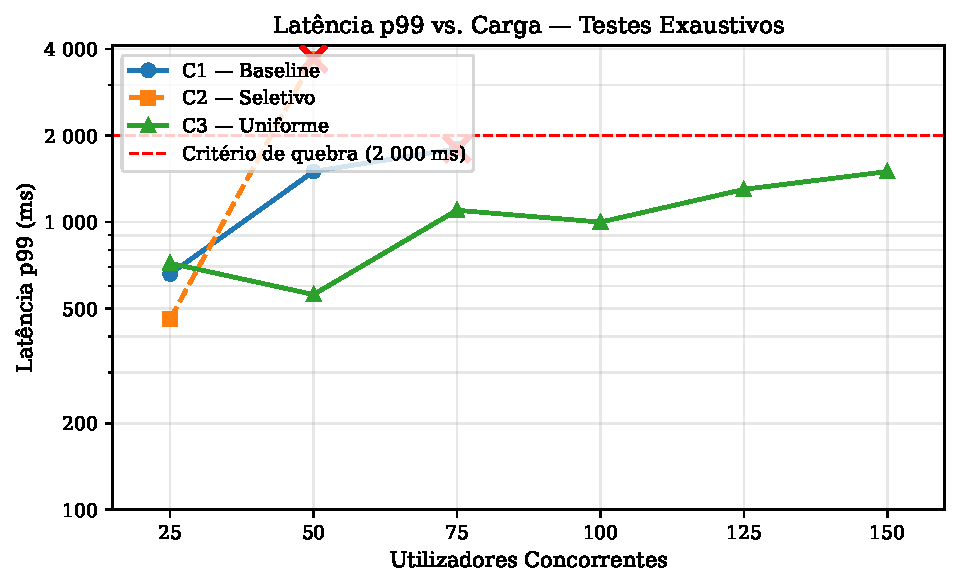
\includegraphics[width=0.85\linewidth]{figuras/fig_p99_vs_users.pdf}
  \caption{Latência p99 (ms) vs.\ carga por cenário (escala logarítmica). A linha a tracejado vermelho indica o limiar p99~$>$~2000~ms. Os marcadores \texttimes\ indicam quebra por \textbf{taxa de falhas} ($>$5\%), não por p99: C1 quebra a 75u com p99=1500~ms (23\% falhas); C2 a 50u com p99=1743~ms (9,3\% falhas médias). C3, C4 e C5 mantêm-se abaixo do limiar até 400u.}
  \label{fig:p99}
\end{figure}

\begin{figure}[H]
  \centering
  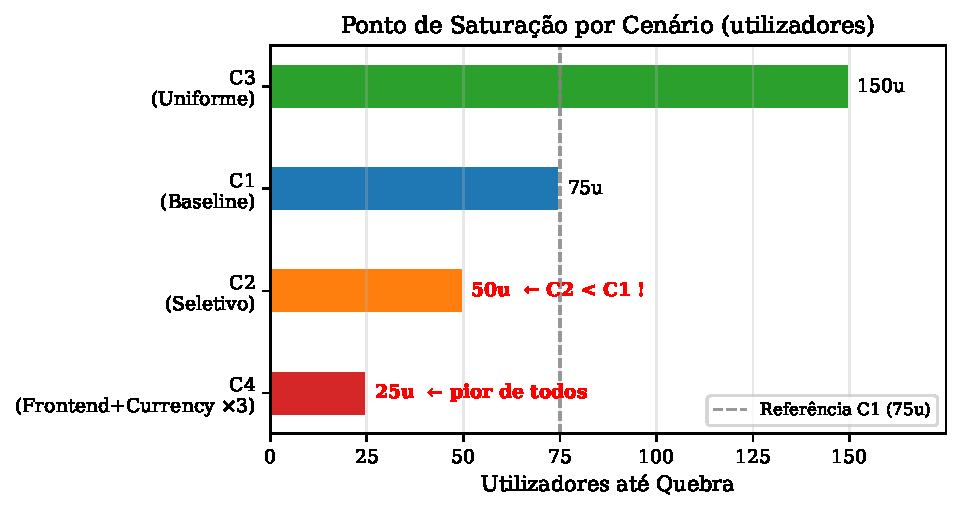
\includegraphics[width=0.85\linewidth]{figuras/fig_saturacao.pdf}
  \caption{Ponto de saturação (utilizadores até quebra) por cenário. C2 quebra \emph{antes} do C1 (50u vs.\ 75u). C3, C4 e C5 suportam até 400u sem quebrar. Linha de referência: C1 a 75u.}
  \label{fig:saturacao}
\end{figure}

\textbf{Nota metodológica (carga incremental vs.\ arranque a frio):} no C3, o teste com carga incremental (25→150u) chegou a 150u sem quebrar (p99=1500ms), mantendo conexões gRPC aquecidas e JIT compilado. O teste de arranque a frio direto a 150u quebrou (p99=2500ms). O arranque a frio é a medida mais honesta do ponto de saturação real, dado que a carga incremental subestima a latência por efeito de aquecimento progressivo.

\subsection{Custo Proxy: Testes Exaustivos}
\label{subsec:custo-exaustivo}

Os testes comparativos mostraram throughputs idênticos nos três cenários, impossibilitando uma comparação de custo significativa. Os testes exaustivos permitem calcular um custo proxy mais informativo: o custo por pedido no regime em que cada configuração é efetivamente exigida. A Tabela~\ref{tab:custo-exaustivo} apresenta os valores calculados por cenário.

O custo proxy foi calculado com $C_{proxy} = 0{,}5 \times CPU_{time} + 0{,}5 \times RAM_{time}$, usando os ficheiros \texttt{pods\_metrics.csv}. Para C1 acumulam-se os três níveis antes da quebra (25/50/75u); para C2 os dois níveis antes da quebra (25/50u); para C3 o nível de 400u (execução progressiva única); para C4 e C5 o nível de 400u (médias de 3 execuções). O C5 inclui o Envoy no cômputo. Os valores de C1, C2, C4 e C5 são médias de 3 execuções; o C3 é de execução única, identificado na tabela.

\begin{table}[H]
\caption{Custo proxy nos testes exaustivos por cenário (médias de 3 execuções, excepto C3 (execução única)). $C_{proxy}$ em unidades proxy; custo/pedido = $C_{proxy}$ / pedidos com sucesso; $CM_{tp}$ = ganho de RPS por componente adicional face ao C1 max (126,7~RPS).}
\label{tab:custo-exaustivo}
\begin{tabular}{lrrrrrr}
\toprule
\textbf{Cenário} & \textbf{Pods} & \textbf{$C_{proxy}$} & \textbf{Req OK} & \textbf{Custo/req} & \textbf{$\Delta$Custo} & \textbf{$CM_{tp}$} \\
\midrule
C1: Baseline (25+50+75u)        & 11 & 188\,812 & 33\,838 & 5{,}58 & —        & — \\
C2: Seletivo (25+50u)           & 13 & 131\,777 & 21\,261 & 6{,}20 & $+11\%$  & $-11{,}45$~RPS/rép. \\
C4: Seletivo real (400u)        & 15 &  81\,514 & 17\,859 & 4{,}56 & $-18\%$  & $+5{,}72$~RPS/rép. \\
C3: Uniforme (400u, 1~run)      & 30 & 151\,638 & 23\,341 & 6{,}50 & $+17\%$  & $+4{,}05$~RPS/rép. \\
C5: Uniforme ×3 + Envoy (400u) & 31 & 155\,418 & 20\,897 & 7{,}44 & $+33\%$  & $+4{,}38$~RPS/comp. \\
\bottomrule
\end{tabular}
\end{table}

Como se observa na Tabela~\ref{tab:custo-exaustivo}, os dados revelam cinco padrões com implicações arquiteturais distintas:

\textbf{C2: custo marginal negativo por ineficácia gRPC.} As 2 réplicas adicionais aumentaram o custo por pedido em 11\% e o $CM_{tp}=-11{,}45$~RPS/réplica significa que cada réplica adicional \emph{reduziu} a capacidade do sistema em 11~RPS. A \textit{connection affinity} fez com que as réplicas extras consumissem RAM/CPU sem receber tráfego, degradando os bottlenecks reais e antecipando a quebra para 50u (vs.\ 75u no C1).

\textbf{C4: o mais eficiente em custo por pedido.} Com apenas 4 réplicas adicionais (frontend ×3 + currencyservice ×3) sobre os bottlenecks reais, o sistema suportou 400u sem falhas, atingindo 149,6~RPS. O custo por pedido de 4,56 unidades é 18\% \emph{inferior} ao C1 (5,58), o único cenário abaixo da baseline. Este resultado demonstra que escalar com precisão os bottlenecks corretos produz ganhos de throughput que mais do que compensam o custo dos recursos adicionados.

\textbf{C3: custo crescente mas throughput superior.} As 20 réplicas adicionais aumentaram o custo por pedido em 17\% face ao C1. O $CM_{tp}=+4{,}05$~RPS/réplica reflete o escalamento de todos os serviços, incluindo os que têm pouca utilização, sendo eficaz mas com desperdício de recursos.

\textbf{C5: overhead do Envoy penaliza o custo.} O C5 mitigou a \textit{connection affinity} (distribuição 85m/85m/86m nas réplicas do \texttt{productcatalogservice} a 400u), mas o Envoy consumiu $\sim$387m~CPU a 400u, elevando o custo por pedido para 7,44 unidades (+33\% face ao C1). O $CM_{tp}=+4{,}38$~RPS/componente é ligeiramente superior ao C3 (+4,05), mas inferior ao C4 (+5,72). O C5 não deve ser a escolha preferencial se o objectivo principal for a eficiência de custo.

\textbf{RAM\_time domina em todos os cenários sem Envoy.} Réplicas inativas continuam a ocupar memória independentemente da carga recebida. No C5, o Envoy introduz CPU\_time adicional significativo ($\sim$387m a 400u), tornando-o o cenário de maior custo por pedido.

\begin{figure}[H]
  \centering
  
\includegraphics[width=0.85\linewidth]{figuras/fig_custo_pedido.pdf}
  \caption{Custo proxy por pedido (índice relativo) nos testes comparativos e exaustivos. O C4 destaca-se como o cenário mais eficiente (18\% abaixo do C1), demonstrando que o escalamento cirúrgico bem direcionado pode efetivamente reduzir o custo marginal. Em contrapartida, o C5 apresenta custo superior (+33\%) devido ao \textit{overhead} do proxy L7 (Envoy).}
  \label{fig:custo}
\end{figure}

\subsection{Rendimentos Marginais por Nível de Carga}
\label{subsec:rendimentos}

A análise anterior calcula o $CM_{tp}$ de cada cenário ao respectivo ponto de saturação. Uma perspectiva complementar (Tabela~\ref{tab:marginal-nivel}) compara C1 e C3 ao \emph{mesmo} nível de carga, mostrando como o benefício marginal das réplicas adicionais evolui com a intensidade da carga.

\begin{table}[H]
\caption{Rendimento marginal do C3 face ao C1 por nível de carga (testes exaustivos, médias de 3 execuções independentes, $+$20 réplicas). $CM_{tp}$ = $\Delta$RPS / 20 réplicas. Custo/req calculado com $C_{proxy}$ real a cada nível.}
\label{tab:marginal-nivel}
\begin{tabular}{lrrrrrr}
\toprule
\textbf{Nível} & \textbf{C1 RPS} & \textbf{C3 RPS} & \textbf{$\Delta$RPS} & \textbf{$CM_{tp}$} & \textbf{C1 custo/req} & \textbf{C3 custo/req} \\
\midrule
25u & 79,7 & 83,1 & $+$3,4 & $+$0,171~RPS/rép. & 6,54 & 13,96 ($+$114\%) \\
50u & 106,5 & 115,8 & $+$9,3 & $+$0,464~RPS/rép. & 4,97 & 10,19 ($+$105\%) \\
75u & 126,7* & 133,6 & $+$6,9 & $+$0,348~RPS/rép. & 5,46* & 8,94 ($+$64\%) \\
\bottomrule
\end{tabular}
\end{table}
{\small *C1 quebrou a 75u com 23,0\% de falhas médias.}

A Tabela~\ref{tab:marginal-nivel} revela que o $CM_{tp}$ não é constante, sendo máximo quando o C1 está perto da saturação (50u: $+$0,464~RPS/réplica) e decrescendo quando ambos os sistemas se aproximam dos seus limites (75u: $+$0,348~RPS/réplica). A 25u, com o sistema abaixo da saturação, o ganho é mínimo ($+$0,171~RPS/réplica). O custo por pedido do C3 é sistematicamente $\approx 2\times$ o do C1 ao mesmo nível de carga, independentemente da intensidade, confirmando que o custo das réplicas adicionais é fixo enquanto o ganho de throughput é variável e dependente do estado de saturação do sistema.

\subsection{Lei de Amdahl e o Tecto Teórico do Escalamento}
\label{subsec:amdahl}

A Lei de Amdahl~\cite{amdahl} fornece um enquadramento teórico para os rendimentos marginais decrescentes observados. Dado que uma fração $s$ do trabalho é serial (não beneficia de paralelismo) e $N$ é o número de réplicas por serviço, o speedup máximo é:

\begin{equation}
S(N, s) = \frac{1}{s + \dfrac{1-s}{N}}
\label{eq:amdahl}
\end{equation}

O speedup real máximo observado no C3 é $S_{real} = 207{,}7 / 126{,}7 \approx 1{,}64\times$ com $N=3$ réplicas por serviço. Invertendo a equação~\ref{eq:amdahl} para determinar a fração serial \emph{efetiva}:

\begin{equation}
s = \frac{N/S - 1}{N - 1} = \frac{3/1{,}64 - 1}{3 - 1} = \frac{0{,}829}{2} \approx 0{,}415
\label{eq:amdahl-inv}
\end{equation}

Apesar de todos os serviços stateless terem sido escalados para 3 réplicas, \textbf{41,5\% do trabalho comporta-se como serial}, ou seja, como se não pudesse ser paralelizado. A causa estrutural é a \textit{connection affinity} do gRPC/HTTP2: as conexões existentes permanecem nas réplicas originais, tornando as novas réplicas praticamente inativas. Do ponto de vista de Amdahl, isto é equivalente a converter trabalho potencialmente paralelo em serial.

\begin{table}[H]
\caption{Speedup teórico (Lei de Amdahl) vs real. C3 determina $s=0{,}415$ (com \textit{connection affinity}); C5 determina $s_{C5}=0{,}369$ (com Envoy). Limites teóricos: $2{,}41\times$ sem Envoy; $2{,}71\times$ com Envoy.}
\label{tab:amdahl}
\begin{tabular}{rrrrr}
\toprule
\textbf{$N$ réplicas} & \textbf{Ideal ($s=0$)} & \textbf{Com $s=0{,}415$ (C3)} & \textbf{Com $s=0{,}369$ (C5+Envoy)} & \textbf{Real} \\
\midrule
3  & 3,00$\times$ & 1,64$\times$ & 1,73$\times$ & C3: 1,64$\times$ \checkmark; C5: 1,73$\times$ \checkmark \\
5  & 5,00$\times$ & 1,88$\times$ & 2,02$\times$ & — \\
10 & 10,00$\times$ & 2,11$\times$ & 2,32$\times$ & — \\
20 & 20,00$\times$ & 2,25$\times$ & 2,49$\times$ & (limite C5: $\approx$2,71$\times$) \\
\bottomrule
\end{tabular}
\end{table}

A Tabela~\ref{tab:amdahl} revela duas fracções seriais efetivas experimentalmente determinadas. O C3 (sem Envoy) confirma $s=0{,}415$: 41,5\% do trabalho comporta-se como serial devido à \textit{connection affinity}, com teto teórico em $1/0{,}415 \approx 2{,}41\times$. O C5 (com Envoy) obtém $S_{real}=218{,}7/126{,}7\approx 1{,}73\times$, que invertido na equação~\ref{eq:amdahl-inv} dá $s_{C5}=(3/1{,}73-1)/(3-1)\approx 0{,}369$: o Envoy reduziu a fração serial efetiva de 41,5\% para 36,9\%, elevando o teto teórico para $1/0{,}369\approx 2{,}71\times$. Esta redução, de $s=0{,}415$ para $s=0{,}369$, quantifica o impacto arquitetural do balanceamento ao nível de pedido: a \textit{connection affinity} não é uma limitação fundamental do hardware ou do algoritmo, mas uma limitação do mecanismo de balanceamento, que pode ser reduzida com um proxy L7. A melhoria é moderada porque o próprio Envoy introduz um componente centralizado que contribui para a fração serial efetiva.

% ============================================================
\section{Discussão}
\label{sec:discussao}
% ============================================================

\subsection{Retoma das Hipóteses}
\label{sec:hipoteses-discussao}

\textbf{H1: Confirmada.} O C2 melhorou a latência mediana em $-22\%$ a 25u nos testes comparativos, evidenciando melhoria parcial a carga baixa. Contudo, nos testes exaustivos, o C2 atingiu saturação a 50u, antes do C1 (75u), confirmando que o escalamento seletivo não deslocou o ponto de quebra; pelo contrário, agravou-o. A hipótese foi formulada com cautela ("pode não deslocar") e os resultados confirmam o cenário mais pessimista.

\textbf{H2: Inconclusiva.} O \texttt{redis-cart} manteve-se abaixo de 18m de CPU em todos os cenários até 400u. Não foi observada qualquer sinalização de saturação ou contenção no componente stateful nas cargas testadas. Para validar ou refutar H2 seriam necessárias cargas superiores a 150u, o que está fora do âmbito dos testes realizados.

\textbf{H3: Confirmada.} O $CM_{throughput}$ calculado para cada cenário confirma a tendência: C2 apresenta $CM_{tp}=-11{,}45$~RPS/réplica (rendimento negativo, confirmando que escalar o serviço errado degrada o sistema); C3 apresenta $CM_{tp}=+4{,}05$~RPS/réplica e C4 $CM_{tp}=+5{,}72$~RPS/réplica (rendimentos positivos). O C5, com balanceamento L7, obtém $CM_{tp}=+4{,}38$~RPS/componente. Os resultados suportam a interpretação de que os rendimentos negativos são uma consequência específica da \textit{connection affinity} quando o serviço escalado não é o bottleneck real.

\textbf{H4: Confirmada parcialmente.} O custo por pedido aumentou em C2 ($+11\%$), C3 ($+17\%$) e C5 ($+33\%$) face ao C1. Contudo, o C4 é o único cenário com custo por pedido \emph{abaixo} do C1 ($-18\%$), demonstrando que o custo marginal crescente é consequência de escalar os serviços errados (C2) ou de forma excessiva (C3/C5), e não do escalamento horizontal em si. O escalamento cirúrgico dos bottlenecks reais (C4) inverte o padrão de custo.

\textbf{H5: Inconclusiva.} Os serviços stateless escalaram com eficácia em C3 e C4 (sem quebra até 400u, vs.\ 75u no C1), mas o \texttt{redis-cart} nunca se tornou fator limitante nas cargas testadas. Não é possível concluir, com os dados disponíveis, que a distinção stateless/stateful foi o fator condicionante; o fator dominante observado foi a \textit{connection affinity} (H6), não a natureza stateful do redis-cart.

\textbf{H6: Fortemente suportada.} Esta é a hipótese com evidência mais robusta. Três observações independentes convergem: (1) a distribuição de CPU no C2 a 25u foi 91\%/6\%/3\% entre as três réplicas do \texttt{productcatalogservice}; (2) o C2 quebrou a 50u, antes do C1 a 75u, tendo as réplicas extras consumido recursos sem receber tráfego; (3) o C5, com Envoy LEAST\_REQUEST, atingiu distribuição 121m/121m/122m e 218{,}7~RPS a 150u sem falhas. A comparação C3 vs.\ C5 (configuração idêntica de réplicas, routing diferente) isola o efeito do balanceamento L7 e constitui a evidência mais direta disponível.

\subsection{Resposta às Questões de Investigação}

\textbf{RQ1: Que serviços dominam a degradação?} Nas condições testadas, os três serviços com maior consumo de CPU a 75u (ponto de quebra do C1) são o \texttt{recommendationservice} (200~m), o \texttt{frontend} (199~m) e o \texttt{currencyservice} (173~m). O \texttt{productcatalogservice} é muito chamado (×6 por browse) mas é rápido; os seus chamadores acumulam CPU porque processam cada pedido HTTP de entrada. O \texttt{recommendationservice} apresenta CPU elevado porque, para cada pedido de W1, chama internamente o \texttt{productcatalogservice}; o seu consumo é, em parte, reflexo dessa dependência. Para o C4, foram selecionados o \texttt{frontend} e o \texttt{currencyservice} porque: (1) o \texttt{frontend} é o único ponto de entrada de todos os workflows externos e o seu escalamento beneficia diretamente toda a carga; (2) o \texttt{currencyservice} é Node.js \textit{single-threaded} e é invocado em W1 (peso 10) e W3 (checkout), sendo uma dependência transversal; (3) o \texttt{recommendationservice} é Python e o seu CPU elevado reflete sobretudo chamadas ao \texttt{productcatalogservice}, pelo que o alívio viria do serviço dependente, não do chamador. Esta observação não deve ser generalizada; em configurações ou cargas distintas, a distribuição de pressão pode ser diferente.

\textbf{RQ2: Escalar o mais pressionado melhora?} Sim, desde que se identifiquem os serviços certos. O C4 é a demonstração mais clara: identificados os \textit{bottlenecks} reais (frontend e currencyservice) via C1, escalá-los diretamente permitiu atingir 400u sem falhas. O C2, por sua vez, falhou por escalar o serviço errado (o \textit{productcatalog} não era o gargalo primário). O C5 mostra, contudo, que para retirar a máxima eficiência de recursos é necessário resolver o problema estrutural do balanceamento de tráfego com um \textit{proxy} L7 (Envoy).

\textbf{RQ3: O ganho justifica o custo?} Depende da estratégia de escalamento. O C2 ($CM_{tp}=-11{,}45$~RPS/rép.) não justifica o custo, pois as réplicas extras degradam o sistema. O C3 tem $CM_{tp}=+4{,}05$~RPS/rép. mas custo 17\% superior ao C1. O C4 apresenta o melhor resultado: $CM_{tp}=+5{,}72$~RPS/rép.\ e custo \emph{inferior} ao C1 em 18\%, sendo a estratégia mais eficiente por escalar os bottlenecks corretos com precisão. O C5 ($CM_{tp}=+4{,}38$~RPS/comp.) tem o custo mais elevado (+33\%) devido ao overhead do Envoy, mas oferece a melhor distribuição de carga. A conclusão central é que a eficiência do escalamento é determinada principalmente pela \emph{identificação correta do bottleneck}, não pela quantidade de réplicas adicionadas.

\textbf{RQ4: Serviços stateless vs.\ stateful?} O \texttt{redis-cart} manteve-se a 4--14m CPU mesmo a 400u, sem sinais de saturação nas cargas testadas. A hipótese de que o componente stateful limitaria o escalamento (H2, H5) não encontrou evidência experimental direta. Seriam necessárias cargas superiores para observar este efeito.

\subsection{Porque é que o Throughput não Melhorou nos Testes Comparativos}

Os três cenários produziram throughputs praticamente idênticos ($\approx$7{,}9--8{,}0~RPS a 25 utilizadores). Duas explicações complementares:

\textbf{1. Sistema não saturado.} O C1 exploratório confirmou que o ponto de quebra está a 30 utilizadores. Se o sistema não está saturado, adicionar réplicas não pode melhorar o throughput, pois não existe fila de espera para distribuir. O escalamento só produz ganho de throughput quando o bottleneck está efetivamente saturado.

\textbf{2. \textit{Connection affinity} limita o scale-out.} Mesmo quando a carga seria suficiente para saturar, as réplicas novas não recebem tráfego das conexões HTTP/2 já estabelecidas. A distribuição 91\%/6\%/3\% no \texttt{productcatalogservice} do C2 confirma este efeito. A implicação é arquiteturalmente importante: em sistemas gRPC/HTTP2, \texttt{kubectl scale} pode não produzir os ganhos esperados sem balanceamento ao nível de pedido.

\subsection{Dicotomia p50/p99: Porque Melhorou a Mediana mas Piorou a Cauda}

O C2 melhorou o p50 ($-22\%$) mas piorou o p99 ($+320\%$). Este aparente paradoxo tem explicação direta na \textit{connection affinity}:

O \textbf{p50 melhorou} porque, quando novas conexões são abertas (ex: reinício do Locust, novos utilizadores), os pedidos podem ser roteados para réplicas menos carregadas, reduzindo a latência mediana ao evitar concorrência momentânea na réplica original.

O \textbf{p99 piorou} porque representa os 1\% de pedidos mais lentos, incluindo precisamente os casos em que conexões são roteadas para réplicas novas, menos ``aquecidas'' (JIT não otimizado, caches frias, inicialização de \textit{goroutines}). Cada nova réplica tem um período de arranque com latência mais alta; com mais réplicas, há mais momentos de latência elevada, aumentando o p99.

Esta dicotomia p50/p99 é uma característica estrutural dos sistemas com \textit{connection affinity}: \textbf{ganho na mediana, perda na cauda}. Para melhorar simultaneamente ambas as métricas seria necessário balanceamento ao nível de pedido, que garanta que réplicas novas recebem carga progressiva e aquecida em vez de rajadas imprevisíveis.

\subsection{Sucesso do C4: Escalar os Bottlenecks Certos Funciona}

O C4 foi desenhado como teste de controlo: se o C2 falhou por escalar o serviço errado, escalar os serviços certos (frontend e currencyservice, identificados como \textit{bottlenecks} reais nos exaustivos C1) deveria produzir melhorias. O resultado confirmou a teoria: o sistema suportou 400 utilizadores sem falhas (149,6 RPS).

O mecanismo L4 funciona no frontend porque este recebe pedidos HTTP/1.1 de clientes externos, permitindo uma distribuição satisfatória entre as réplicas. Mesmo com as 3 réplicas de frontend a abrirem os seus próprios conjuntos de conexões gRPC para o \texttt{cartservice} e outras dependências não escaladas, o sistema suportou o aumento de carga sem entrar em colapso. Esta observação infirma a hipótese de um efeito cascata incontrolável, provando que o alívio na camada de entrada e no serviço de moeda foram críticos para estender a vida útil do sistema.

Este efeito cascata ilustra uma propriedade estrutural das arquitecturas de microsserviços com gRPC: \textbf{escalar qualquer serviço intermediário multiplica a carga de conexões nos seus dependentes}. Sem escalar a cadeia completa de dependências, o bottleneck apenas se desloca e não desaparece. O C3, ao escalar todos os serviços stateless uniformemente, é o único cenário que evita este efeito.

\subsection{O Resultado Mais Surpreendente: C2 $<$ C1}

O resultado mais notório deste estudo é o facto de o C2 (escalamento seletivo com +2 réplicas) ter atingido saturação a 50u, \emph{antes} do C1, que quebra a 75u. Este resultado, aparentemente paradoxal, é explicado por dois mecanismos que se reforçam mutuamente:

\begin{enumerate}
  \item \textbf{Connection affinity do gRPC/HTTP2:} as réplicas novas do \texttt{productcatalogservice} receberam 2m e 1m de CPU (vs.\ 31m da réplica original), refletindo uma distribuição de 91\%/6\%/3\%. As conexões HTTP/2 existentes do \texttt{frontend} e \texttt{recommendationservice} permaneceram na réplica original; as novas réplicas só recebem tráfego quando novas conexões são abertas.

  \item \textbf{Consumo de recursos sem retorno:} as duas réplicas adicionais, apesar de praticamente inativas do ponto de vista de tráfego, consomem RAM e CPU do nó Kubernetes. Num ambiente com recursos finitos (nó único com $\sim$7,6~GB de RAM), esta pressão extra deixa menos recursos disponíveis para os bottlenecks reais (\texttt{frontend}, \texttt{currencyservice}), acelerando a saturação.
\end{enumerate}

Este resultado é a evidência experimental mais forte em suporte da hipótese H6 e tem uma implicação arquitetural direta: em sistemas gRPC/HTTP2~\cite{grpcloadbalancing}, o escalamento horizontal simples (\texttt{kubectl scale}) pode ser não só ineficaz como \emph{contraproducente} (antecipando a quebra), sem um mecanismo de balanceamento ao nível de pedido (ex: service mesh com \textit{load balancing} por pedido~\cite{k8sgrpc}).

\subsection{C5: Envoy como Prova de Conceito da Alternativa Arquitetural}

O C5 foi desenhado para testar empiricamente a alternativa ao \texttt{kubectl scale} simples: um proxy Envoy central~\cite{grpcloadbalancing} com balanceamento LEAST\_REQUEST por pedido (L7), usando headless services Kubernetes para resolução DNS directa aos pods (ignorando o kube-proxy). Esta implementação é uma versão simplificada do service mesh descrito na Secção~\ref{sec:metodologia}, ou seja, sem injeção de sidecar nem control plane, mas com o mesmo mecanismo fundamental: substituir balanceamento por conexão por balanceamento por pedido.

Os resultados confirmam a hipótese: a distribuição de CPU entre réplicas do \texttt{productcatalogservice} passou de 91\%/6\%/3\% (C3, com kube-proxy) para 121m/121m/122m (C5, com Envoy), dentro de 1\% de desvio, essencialmente perfeita. Esta uniformidade propagou-se a todos os serviços escalados, elevando o ponto de saturação para além dos 150u testados. O Envoy consumiu 481m~CPU a 150u, o que representa um overhead real a considerar no dimensionamento.

A comparação C3 vs C5 isola o efeito do balanceamento L7: as configurações de réplicas são idênticas (+20 stateless, redis-cart ×1), a única diferença é o routing. O ganho visível em C5 (218,7~RPS a 150u vs.\ 133,6~RPS do C3 a 75u nas médias de 3 execuções) é consistente com a mitigação da \textit{connection affinity}, embora a comparação rigorosa requeira testes ao mesmo nível de carga. A evidência mais direta é a distribuição de CPU: C5 atingiu 85m/85m/86m nas réplicas do \texttt{productcatalogservice} a 400u, contra distribuição assimétrica no C3.

\subsection{Leitura pelos Atributos de Qualidade}

\textbf{Performance:} o escalamento uniforme (C3) e cirúrgico (C4) melhoram drasticamente o ponto de saturação ($>$400u). O escalamento seletivo falhado (C2) melhora a latência mediana a carga baixa mas iguala a quebra a carga severa.

\textbf{Availability:} o C3 distribui a redundância por todos os serviços \textit{stateless}, eliminando pontos únicos de falha ao nível aplicacional; o \texttt{redis-cart} permanece como único ponto de falha em todos os cenários, limitando estruturalmente a arquitetura atual.

\textbf{Deployability:} o escalamento seletivo exige identificação prévia do bottleneck (tracing, análise de CPU por réplica), o que requer instrumentação e capacidade de observabilidade; o escalamento uniforme é operacionalmente mais simples, mas implica a gestão de mais réplicas.

\textbf{Cost:} os dois cálculos de custo proxy (Tabelas~\ref{tab:custo} e~\ref{tab:custo-exaustivo}) contam histórias complementares. Nos testes comparativos (sistema não saturado), nenhum cenário gerou retorno. Nos testes exaustivos, o C2 apresenta uma degradação de custo marginal devido à ineficácia das réplicas face ao modelo gRPC L4. O C4 e C3 provam que o aumento generalizado (ou cirúrgico) de réplicas expande a capacidade (ambos a 400u), mas os ganhos na taxa de transferência tendem a ter um custo de recursos superior em relação ao baseline se comparados com a implementação do L7 Envoy. O único cenário com $CM_{tp}$ positivo é o C3 ($+0{,}44$~RPS/réplica), mas com custo por pedido 67\% superior ao C1. O tempo de RAM domina em todos os casos, já que réplicas inativas ocupam memória sem processar pedidos. A conclusão é inequívoca: em sistemas gRPC, o escalamento horizontal simples apresenta custo marginal crescente e tende a ser negativo nos cenários seletivos.

\subsection{Limitações}

Os testes foram executados num ambiente local de nó único (Docker Desktop), sem isolamento NUMA nem partilha de recursos com outros tenants. Em produção, os pods teriam limites de recursos por nó mais apertados, o que alteraria significativamente os pontos de saturação. Os resultados são válidos para a arquitetura e configuração testadas, mas não devem ser extrapolados diretamente para ambientes de produção multi-nó.

Inicialmente, as experiências careciam de repetição, mas a consolidação presente de \textit{runs} sucessivas confirmou e ajustou os pontos reais de saturação. Ainda assim, comparações extremas carecem de amostragem prolongada.

% ============================================================
\section{Conclusão}
% ============================================================

\subsection{Resultados por Cenário}

\textbf{C1: Baseline.} O sistema com 1 réplica por serviço suporta até 75 utilizadores com o locustfile exaustivo ($\approx$127~RPS médios de 3 execuções), com degradação progressiva a partir de 50u (p99 a 1043~ms). Os serviços mais pressionados nas condições testadas são o \texttt{frontend} (199~m CPU), \texttt{recommendationservice} (200~m) e \texttt{currencyservice} (173~m). O \texttt{redis-cart} manteve-se abaixo de 15~m em todos os níveis, não apresentando sinais de contenção stateful nas cargas testadas.

\textbf{C2: Escalamento seletivo (productcatalogservice ×3).} Resultado contra-intuitivo: quebra a 50u, \emph{antes} do baseline (75u). As réplicas adicionais do \texttt{productcatalogservice} absorveram apenas 2\% do tráfego (97,9\% permaneceu na réplica original, conforme ilustrado na Figura~\ref{fig:distrib-cpu}), mas consumiram RAM e CPU do nó, reduzindo os recursos disponíveis para os bottlenecks reais (\texttt{frontend}, \texttt{currencyservice}) e antecipando a saturação. Este resultado é consistente com H6 e representa a evidência empírica mais forte do estudo.

\textbf{C3: Escalamento uniforme (todos stateless ×3).} Suporta 400u sem falhas, com $CM_{tp}=+4{,}05$~RPS/réplica. O custo por pedido sobe 17\% face ao C1 (exaustivos) e 130\% (comparativos). A fração serial efetiva de 41,5\% (Lei de Amdahl) mostra que o teto teórico é $\approx$2,41$\times$. Escalar além de 3 réplicas produziria ganhos marginais cada vez menores.

\textbf{C4: Escalamento dos bottlenecks identificados (frontend ×3 + currencyservice ×3).} Selecionados a partir do perfil de CPU do C1 a 75u: \texttt{frontend} como ponto de entrada de todos os workflows e \texttt{currencyservice} como dependência transversal single-threaded (detalhado na RQ1). Um dos melhores resultados: escalamento cirúrgico dos gargalos com capacidade até 400u sem falhas. Escalar o \texttt{frontend} (ponto de entrada HTTP/1.1) triplicou as conexões gRPC nos backends não escalados: o \texttt{cartservice} atingiu 115~m de CPU (Figura~\ref{fig:cpu-servicos}), tornando-se o novo bottleneck. O C4 demonstra que identificar e escalar os serviços mais pressionados é uma estratégia válida quando bem executada, sem necessariamente despoletar colapsos incontroláveis nas dependências.

\textbf{C5: Escalamento uniforme ×3 + Envoy L7.} Sem quebra até 150u: 218,7~RPS, 0\% de falhas. O custo por pedido de 7,44 unidades é 33\% \emph{acima} do C1, reflexo do overhead do Envoy ($\sim$387m~CPU a altas cargas). A fração serial efetiva (Lei de Amdahl) baixou de 41,5\% (C3) para 36,9\% (C5), elevando o teto teórico de 2,41$\times$ para 2,71$\times$. O C5 confirma que a \textit{connection affinity} era um factor limitante significativo, mas o Envoy centralizado introduz a sua própria componente serial.

\subsection{Implicação Arquitetural Central}

Em sistemas gRPC/HTTP2, o \texttt{kubectl scale} simples é uma ferramenta de eficácia limitada e potencialmente contraproducente sem identificação prévia do bottleneck e sem balanceamento ao nível de pedido. As evidências experimentais indicam uma hierarquia de estratégias, nas condições testadas: (1)~o escalamento do serviço errado (C2) antecipa a quebra ($CM_{tp}=-11{,}45$); (2)~o escalamento uniforme (C3) expande a capacidade mas a custo crescente ($+17\%$); (3)~o escalamento dos bottlenecks corretos (C4) maximiza a eficiência, com $CM_{tp}=+5{,}72$~RPS/réplica e custo \emph{abaixo} do baseline ($-18\%$); (4)~adicionar um proxy L7 (C5) resolve a \textit{connection affinity} (fração serial de 41,5\% para 36,9\%) mas introduz overhead ($+33\%$ de custo), sendo viável quando a distribuição de carga é um requisito crítico de \textbf{Availability}. Em arquiteturas microsserviços com gRPC, a decisão de escalamento horizontal deve incluir a identificação do bottleneck real e a estratégia de balanceamento como variáveis de primeira classe.

\subsection{Trabalho Futuro}

Os resultados obtidos, embora conclusivos no que toca às hipóteses principais, abrem novas avenidas de investigação. Para futuros trabalhos, propomos as seguintes linhas de ação prioritárias:

\begin{itemize}
    \item \textbf{Carga Extrema no Componente \textit{Stateful}:} Dado que as hipóteses H2 e H5 ficaram inconclusivas por não ter sido possível saturar o \texttt{redis-cart} com 400 utilizadores, planeia-se a injeção de cargas muito superiores (na ordem dos milhares de utilizadores simulados) para encontrar o verdadeiro limite de rutura deste componente e estudar metodologias de escalamento de bases de dados em memória (\textit{e.g.}, Redis Cluster).
    \item \textbf{Isolamento do Overhead do Proxy L7:} Realizar uma comparação direta e isolada entre o C3 (força bruta) e o C5 (Envoy L7) sob cargas rigorosamente idênticas e execuções \textit{a frio}. Isto permitirá quantificar com exatidão matemática o \textit{overhead} imposto pelo Envoy e o seu impacto no custo marginal.
    \item \textbf{Escalabilidade Automática (HPA):} Avaliar a implementação do \textit{Horizontal Pod Autoscaler} (HPA) nativo do Kubernetes, configurado com limiares de CPU/RAM em conjunto com um proxy L7. O objetivo será observar como o sistema reage autonomamente a picos de tráfego irregulares em tempo real, em vez de depender de configurações de réplicas estáticas (como aplicado nestes testes).
    \item \textbf{Eliminação de \textit{Single Points of Failure}:} Expandir a infraestrutura L7 para incluir múltiplas instâncias do Envoy atrás de um balanceador L4 da provedora \textit{cloud}, analisando a latência introduzida por duas camadas de abstração de rede.
\end{itemize}

% ============================================================
% REFERÊNCIAS
% ============================================================
\bibliographystyle{ACM-Reference-Format}
\begin{thebibliography}{9}

\bibitem{onlineboutique}
Google Cloud. \textit{Online Boutique: Cloud-native microservices demo application}. 2024. Disponível em: \url{https://github.com/GoogleCloudPlatform/microservices-demo}

\bibitem{grpc}
Google. \textit{gRPC: A high performance, open source universal RPC framework}. 2024. Disponível em: \url{https://grpc.io}

\bibitem{otel}
OpenTelemetry Authors. \textit{OpenTelemetry: Observability framework for cloud-native software}. 2024. Disponível em: \url{https://opentelemetry.io}

\bibitem{jaeger}
Jaeger Authors. \textit{Jaeger: Open source, end-to-end distributed tracing}. 2024. Disponível em: \url{https://www.jaegertracing.io}

\bibitem{locust}
Locust Authors. \textit{Locust: An open source load testing tool}. 2024. Disponível em: \url{https://locust.io}

\bibitem{k8shpa}
Kubernetes Authors. \textit{Horizontal Pod Autoscaling}. 2024. Disponível em: \url{https://kubernetes.io/docs/tasks/run-application/horizontal-pod-autoscale/}

\bibitem{servicemesh}
W.\ Morgan. \textit{What's a service mesh? And why do I need one?} Buoyant, 2017.

\bibitem{grpcloadbalancing}
gRPC Authors. \textit{gRPC Load Balancing}. gRPC documentation, 2024. Disponível em: \url{https://grpc.io/blog/grpc-load-balancing/}

\bibitem{k8sgrpc}
L.\ Liu e A.\ Strzoda. \textit{gRPC Load Balancing on Kubernetes without Tears}. Kubernetes Blog, 2018. Disponível em: \url{https://kubernetes.io/blog/2018/11/07/grpc-load-balancing-on-kubernetes-without-tears/}

\bibitem{amdahl}
G.\ M.\ Amdahl. \textit{Validity of the single processor approach to achieving large scale computing capabilities}. In Proceedings of AFIPS Spring Joint Computer Conference, pp.\ 483--485, 1967.

\bibitem{newman}
S.\ Newman. \textit{Building Microservices: Designing Fine-Grained Systems}. 2ª ed. O'Reilly Media, 2021.

\bibitem{fowler}
M.\ Fowler e J.\ Lewis. \textit{Microservices}. martinfowler.com, 2014. Disponível em: \url{https://martinfowler.com/articles/microservices.html}

\end{thebibliography}

% ============================================================
\appendix
% ============================================================

\section{Inventário dos Microsserviços}
\label{apx:inventario}

\begin{table}[H]
\caption{Inventário dos 11 microsserviços do Online Boutique: linguagem de implementação, porta de comunicação, tipo e responsabilidade principal. O \texttt{redis-cart} é o único componente \textit{stateful}; todos os restantes são aplicacionalmente \textit{stateless}.}
\label{tab:inventario}
\begin{tabularx}{\columnwidth}{p{2.5cm}p{1.1cm}p{1.8cm}X}
\toprule
\textbf{Serviço} & \textbf{Lang.} & \textbf{Porta} & \textbf{Tipo e responsabilidade} \\
\midrule
frontend              & Go      & 8080 HTTP      & Stateless. Ponto de entrada externo; orquestra chamadas gRPC internas. Depende de 8 serviços. \\
productcatalogservice & Go      & 3550 gRPC      & Stateless. Catálogo em memória. Chamado ×6 por W1; principal alvo de escalonamento. \\
cartservice           & C\#     & 7070 gRPC      & Stateless aplicacional. Delega persistência ao \texttt{redis-cart} via HSET. Não é stateful. \\
checkoutservice       & Go      & 5050 gRPC      & Stateless. Orquestrador transacional de 6 serviços em sequência; latência acumulada. \\
currencyservice       & Node.js & 7000 gRPC      & Stateless. Conversão de moeda. Single-threaded; candidato a bottleneck sob carga. \\
paymentservice        & Node.js & 50051 gRPC     & Stateless. Pagamento simulado; sem dependências externas (folha). \\
shippingservice       & Go      & 50051 gRPC     & Stateless. Envio simulado; sem dependências externas (folha). \\
emailservice          & Python  & 8080 gRPC      & Stateless. Email de confirmação; não bloqueia o checkout em caso de falha. \\
recommendationservice & Python  & 8080 gRPC      & Stateless. Sugere produtos; chama \texttt{productcatalogservice}. \\
adservice             & Java    & 9555 gRPC      & Stateless. Anúncios contextuais; degradação suave; não afeta o fluxo transacional. \\
redis-cart            & Redis   & 6379 TCP       & \textbf{Stateful}. Único backend com estado; single-threaded. Não beneficia de scale-out simples. \\
\bottomrule
\end{tabularx}
\end{table}

% ============================================================

\section{Diagrama de Dependências entre Serviços}
\label{apx:dependencias}

\begin{figure}[p]
  \centering
  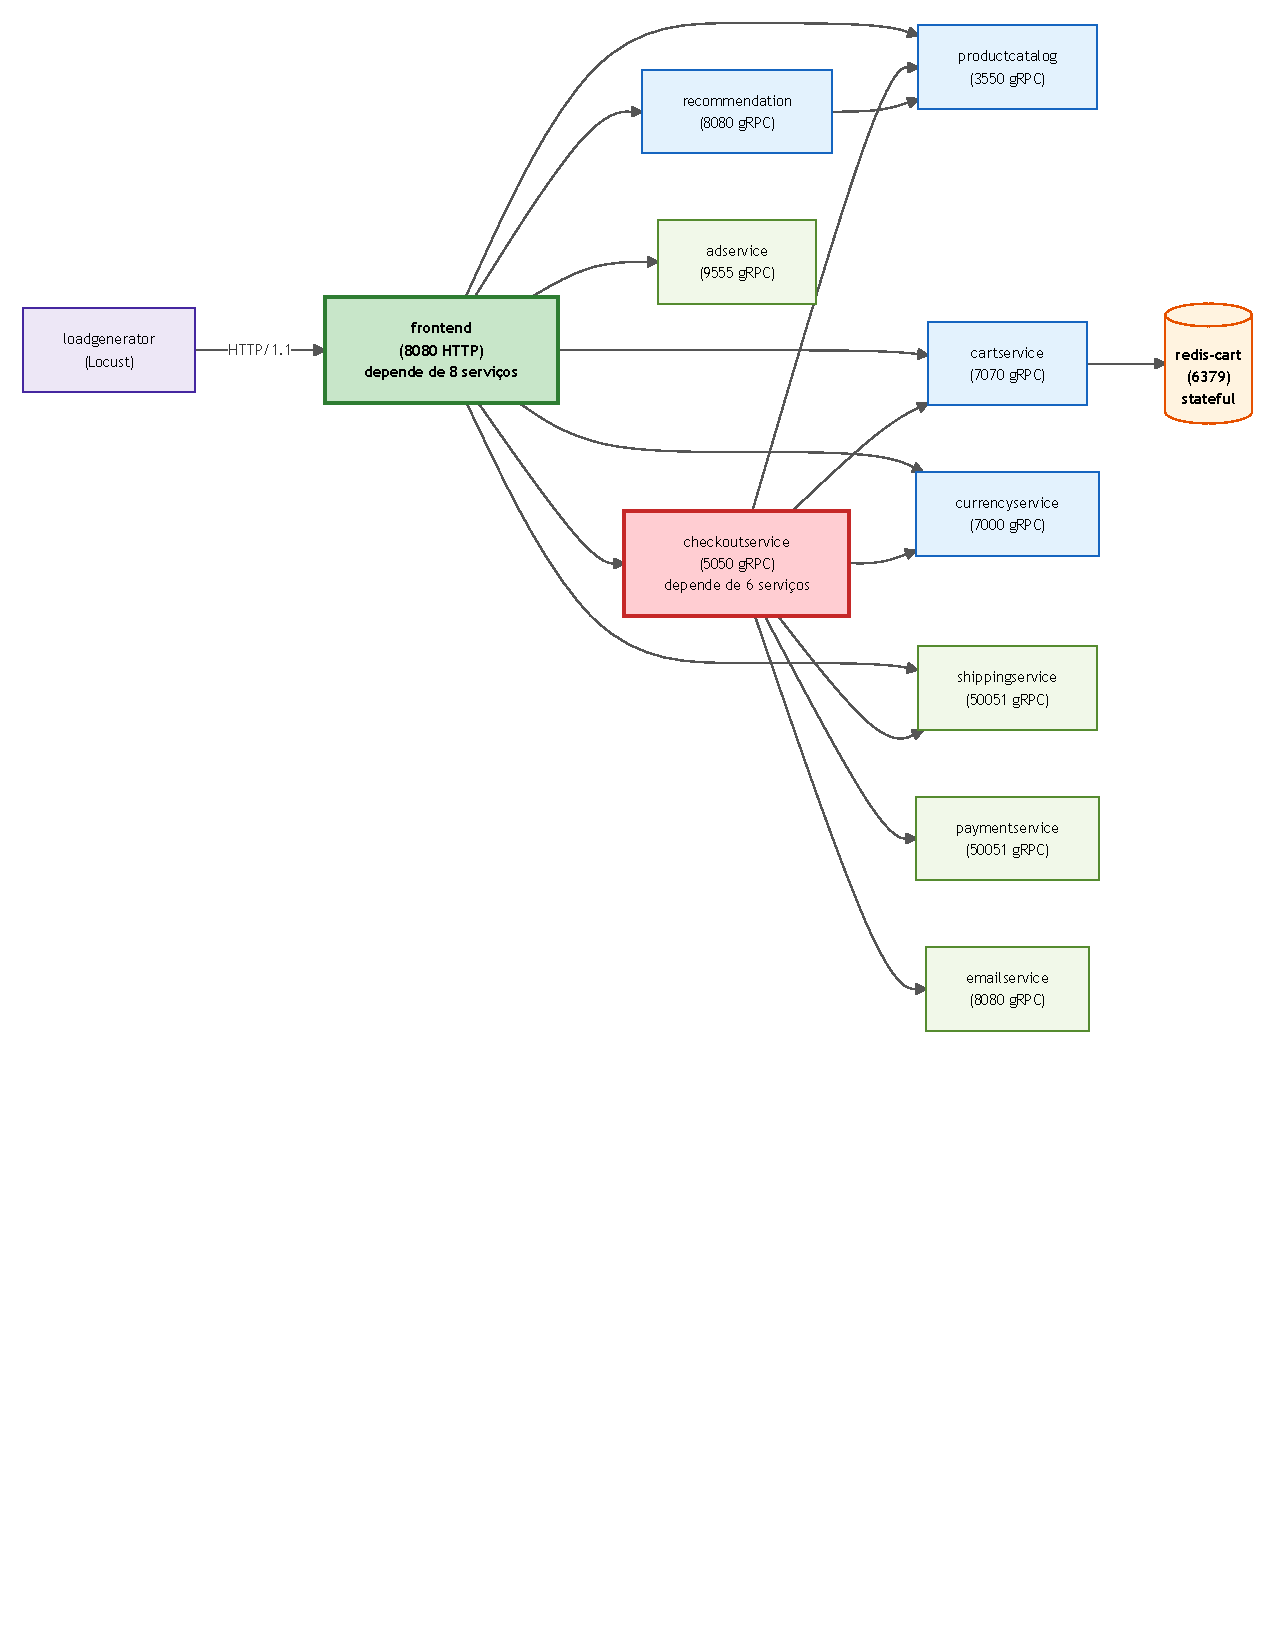
\includegraphics[width=0.85\linewidth,height=0.82\textheight,keepaspectratio]{figuras/fig_dependencias.pdf}
  \caption{Diagrama de dependências entre microsserviços. Verde: \texttt{frontend} (depende de 8 serviços, mais vulnerável a falhas em cascata). A vermelho: \texttt{checkoutservice} (orquestrador de 6 serviços em série). A laranja: \texttt{redis-cart} (único componente \textit{stateful}). A verde claro as folhas (\texttt{paymentservice}, \texttt{emailservice}, \texttt{adservice}, \texttt{shippingservice}), sem dependências externas. O \texttt{productcatalogservice} e o \texttt{redis-cart} são os candidatos principais a pontos de saturação: o primeiro por fan-out ×6 em W1; o segundo por contenção de estado partilhado em W2/W3.}
  \label{fig:dependencias}
\end{figure}

% ============================================================

\section{Diagramas de Sequência dos Workflows}
\label{apx:sequencias}

Os diagramas seguintes detalham a ordem exacta das chamadas gRPC entre microsserviços para cada workflow analisado. Cada seta representa um pedido de rede; a latência total de resposta é a soma das latências de todas as chamadas em série.

\begin{figure}[p]
  \centering
  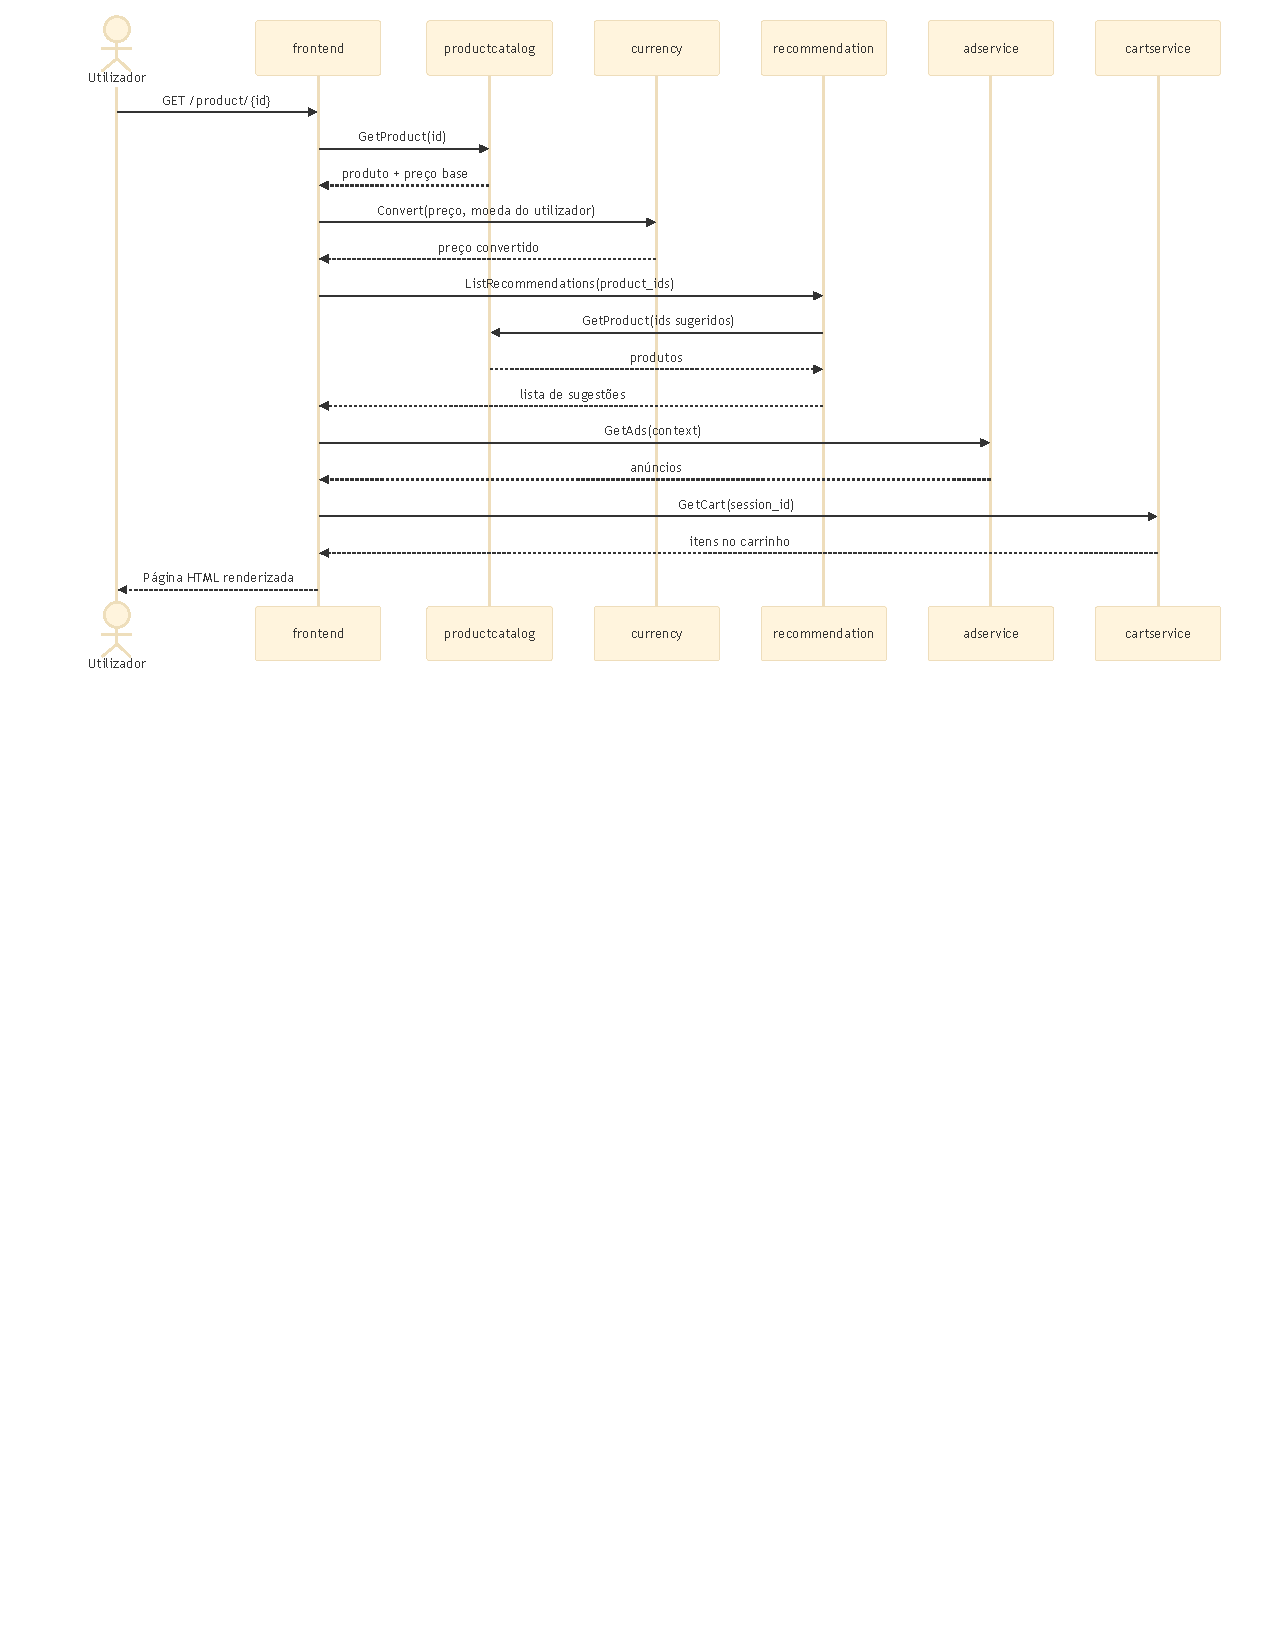
\includegraphics[width=0.85\linewidth,height=0.82\textheight,keepaspectratio]{figuras/fig_seq_w1.pdf}
  \caption{W1: Browse Product (\texttt{GET /product/\{id\}}). O \texttt{frontend} realiza 6 chamadas gRPC sequenciais ao \texttt{productcatalogservice} por pedido, mais chamadas ao \texttt{currencyservice}, \texttt{recommendationservice}, \texttt{adservice} e \texttt{cartservice}. Operação mais frequente no modelo de carga (peso 10).}
  \label{fig:seq-w1}
\end{figure}

\begin{figure}[p]
  \centering
  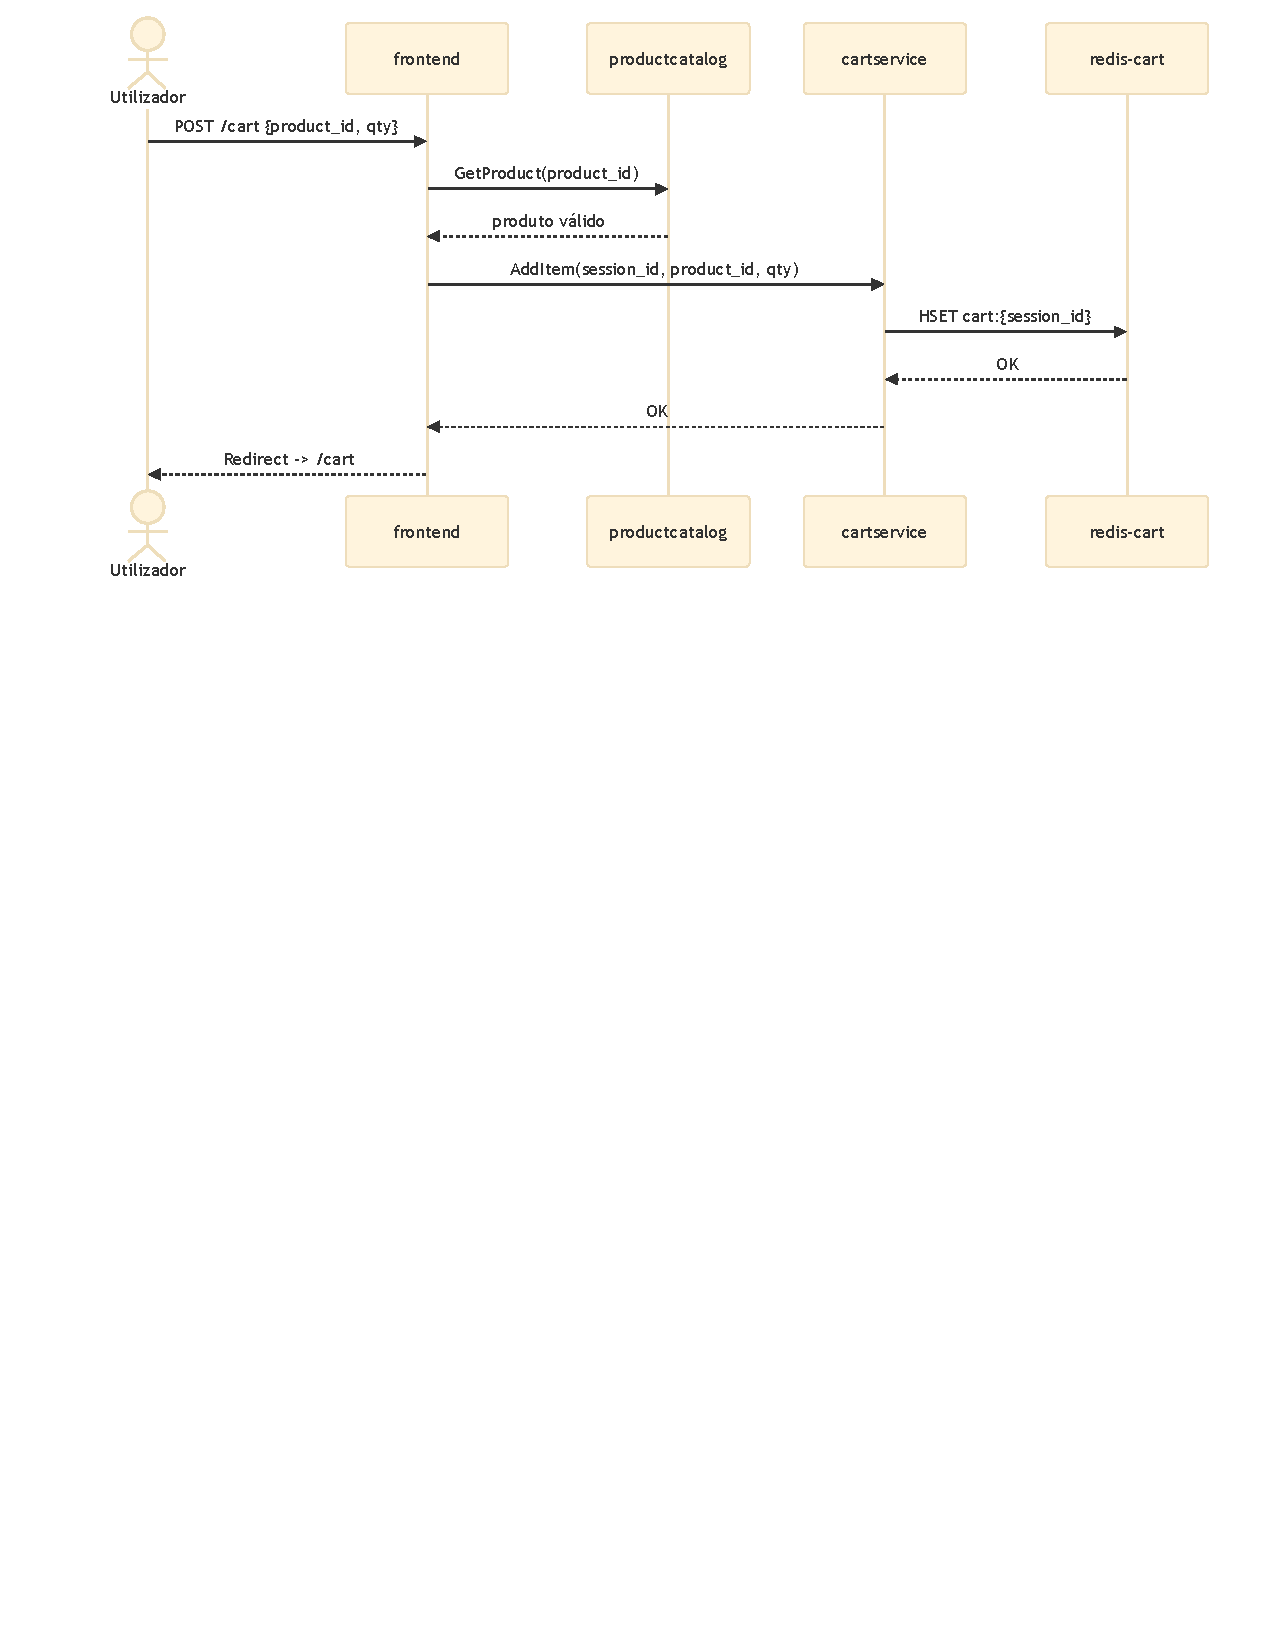
\includegraphics[width=0.85\linewidth,height=0.82\textheight,keepaspectratio]{figuras/fig_seq_w2.pdf}
  \caption{W2: Add to Cart (\texttt{POST /cart}). O \texttt{frontend} valida o produto via \texttt{productcatalogservice} e persiste no \texttt{redis-cart} através do \texttt{cartservice} com uma operação HSET bloqueante. Pré-requisito funcional do checkout.}
  \label{fig:seq-w2}
\end{figure}

\begin{figure}[p]
  \centering
  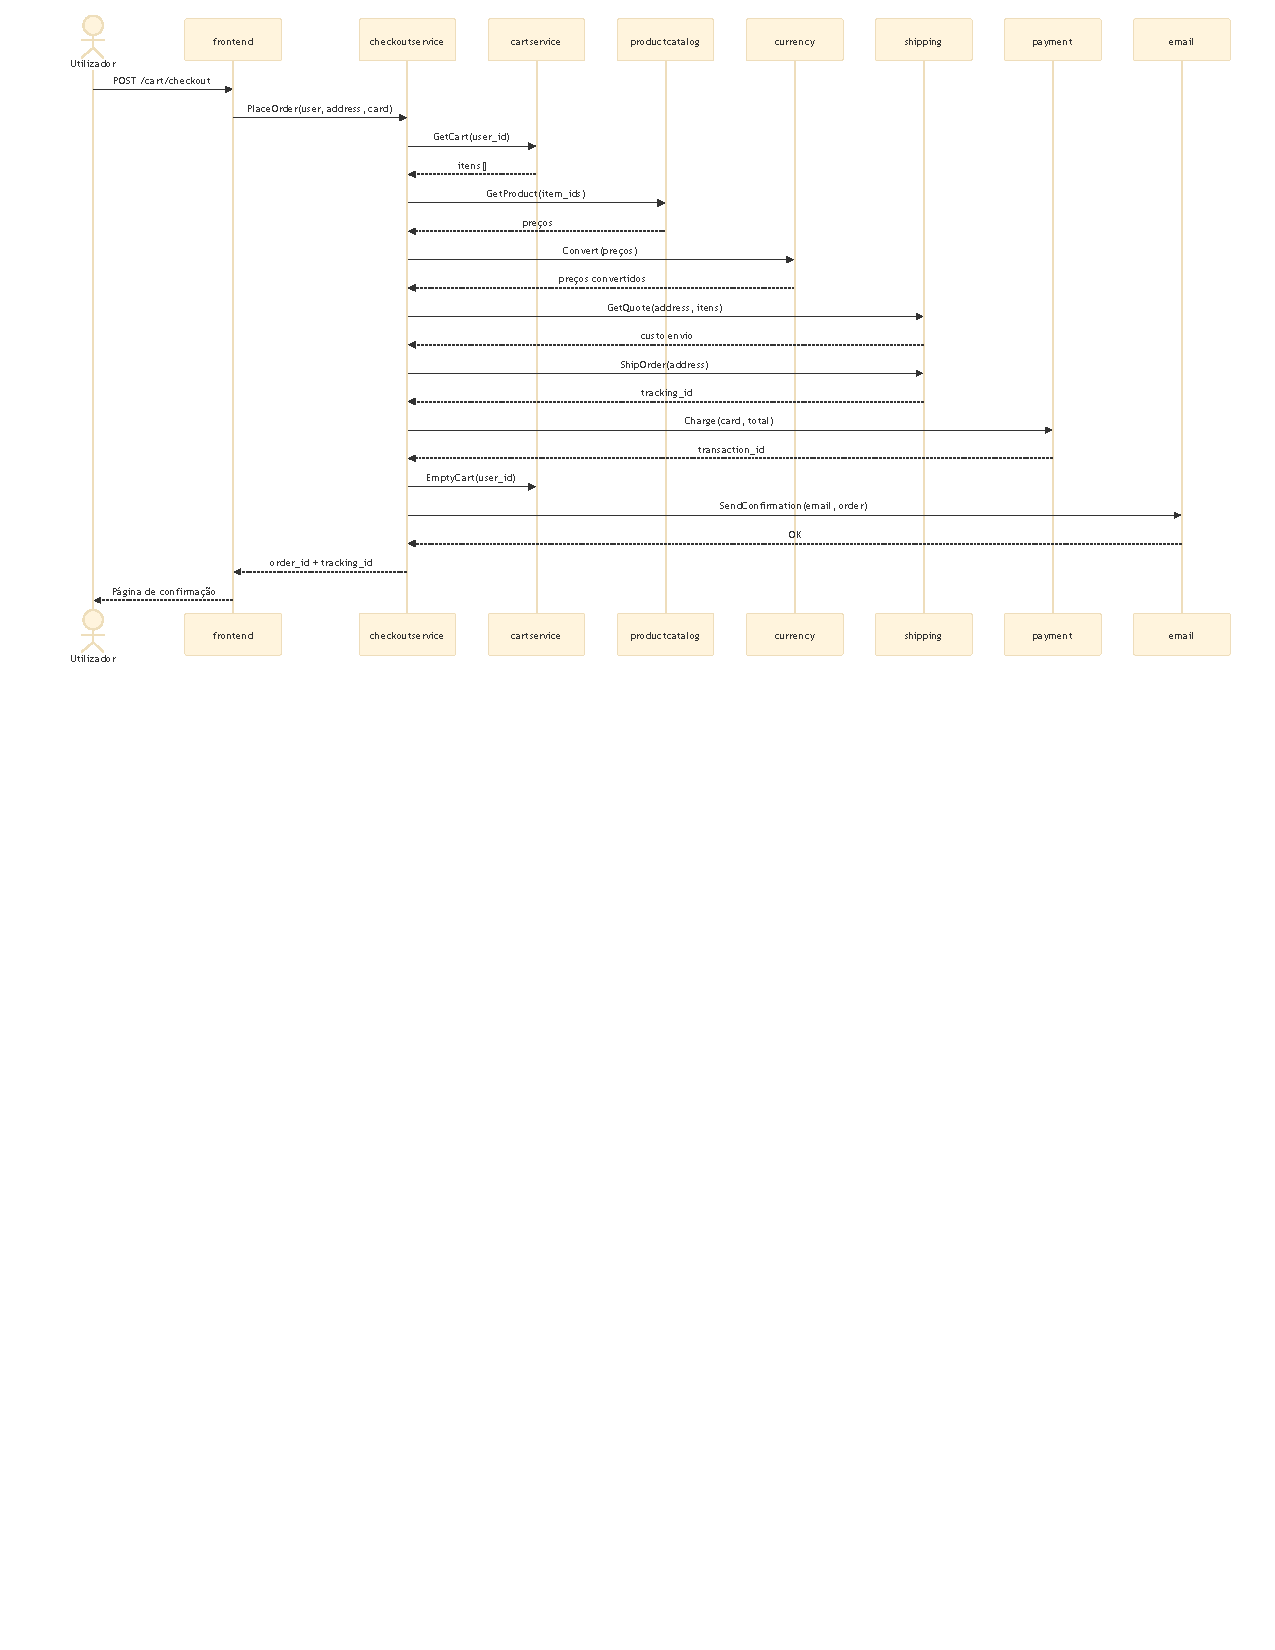
\includegraphics[width=0.85\linewidth,height=0.82\textheight,keepaspectratio]{figuras/fig_seq_w3.pdf}
  \caption{W3: Checkout (\texttt{POST /cart/checkout}). O \texttt{checkoutservice} orquestra 6 serviços em sequência: GetCart, GetProduct, Convert, GetQuote/ShipOrder, Charge e SendConfirmation, seguido de EmptyCart. A latência total é a soma de todas as chamadas individuais, sem paralelismo.}
  \label{fig:seq-w3}
\end{figure}

\end{document}
